\chapter[Appendix: Splitting Sequences for the Stratum]{Appendix: Splitting Sequences for the Stratum}
\label{app:splitting_big_stratum}


\begin{figure*}[p] % [p] forces this to be on its own page, which is often necessary for large figures
    \centering
    % Restrict height to 45% of the text block per image, maintaining aspect ratio
    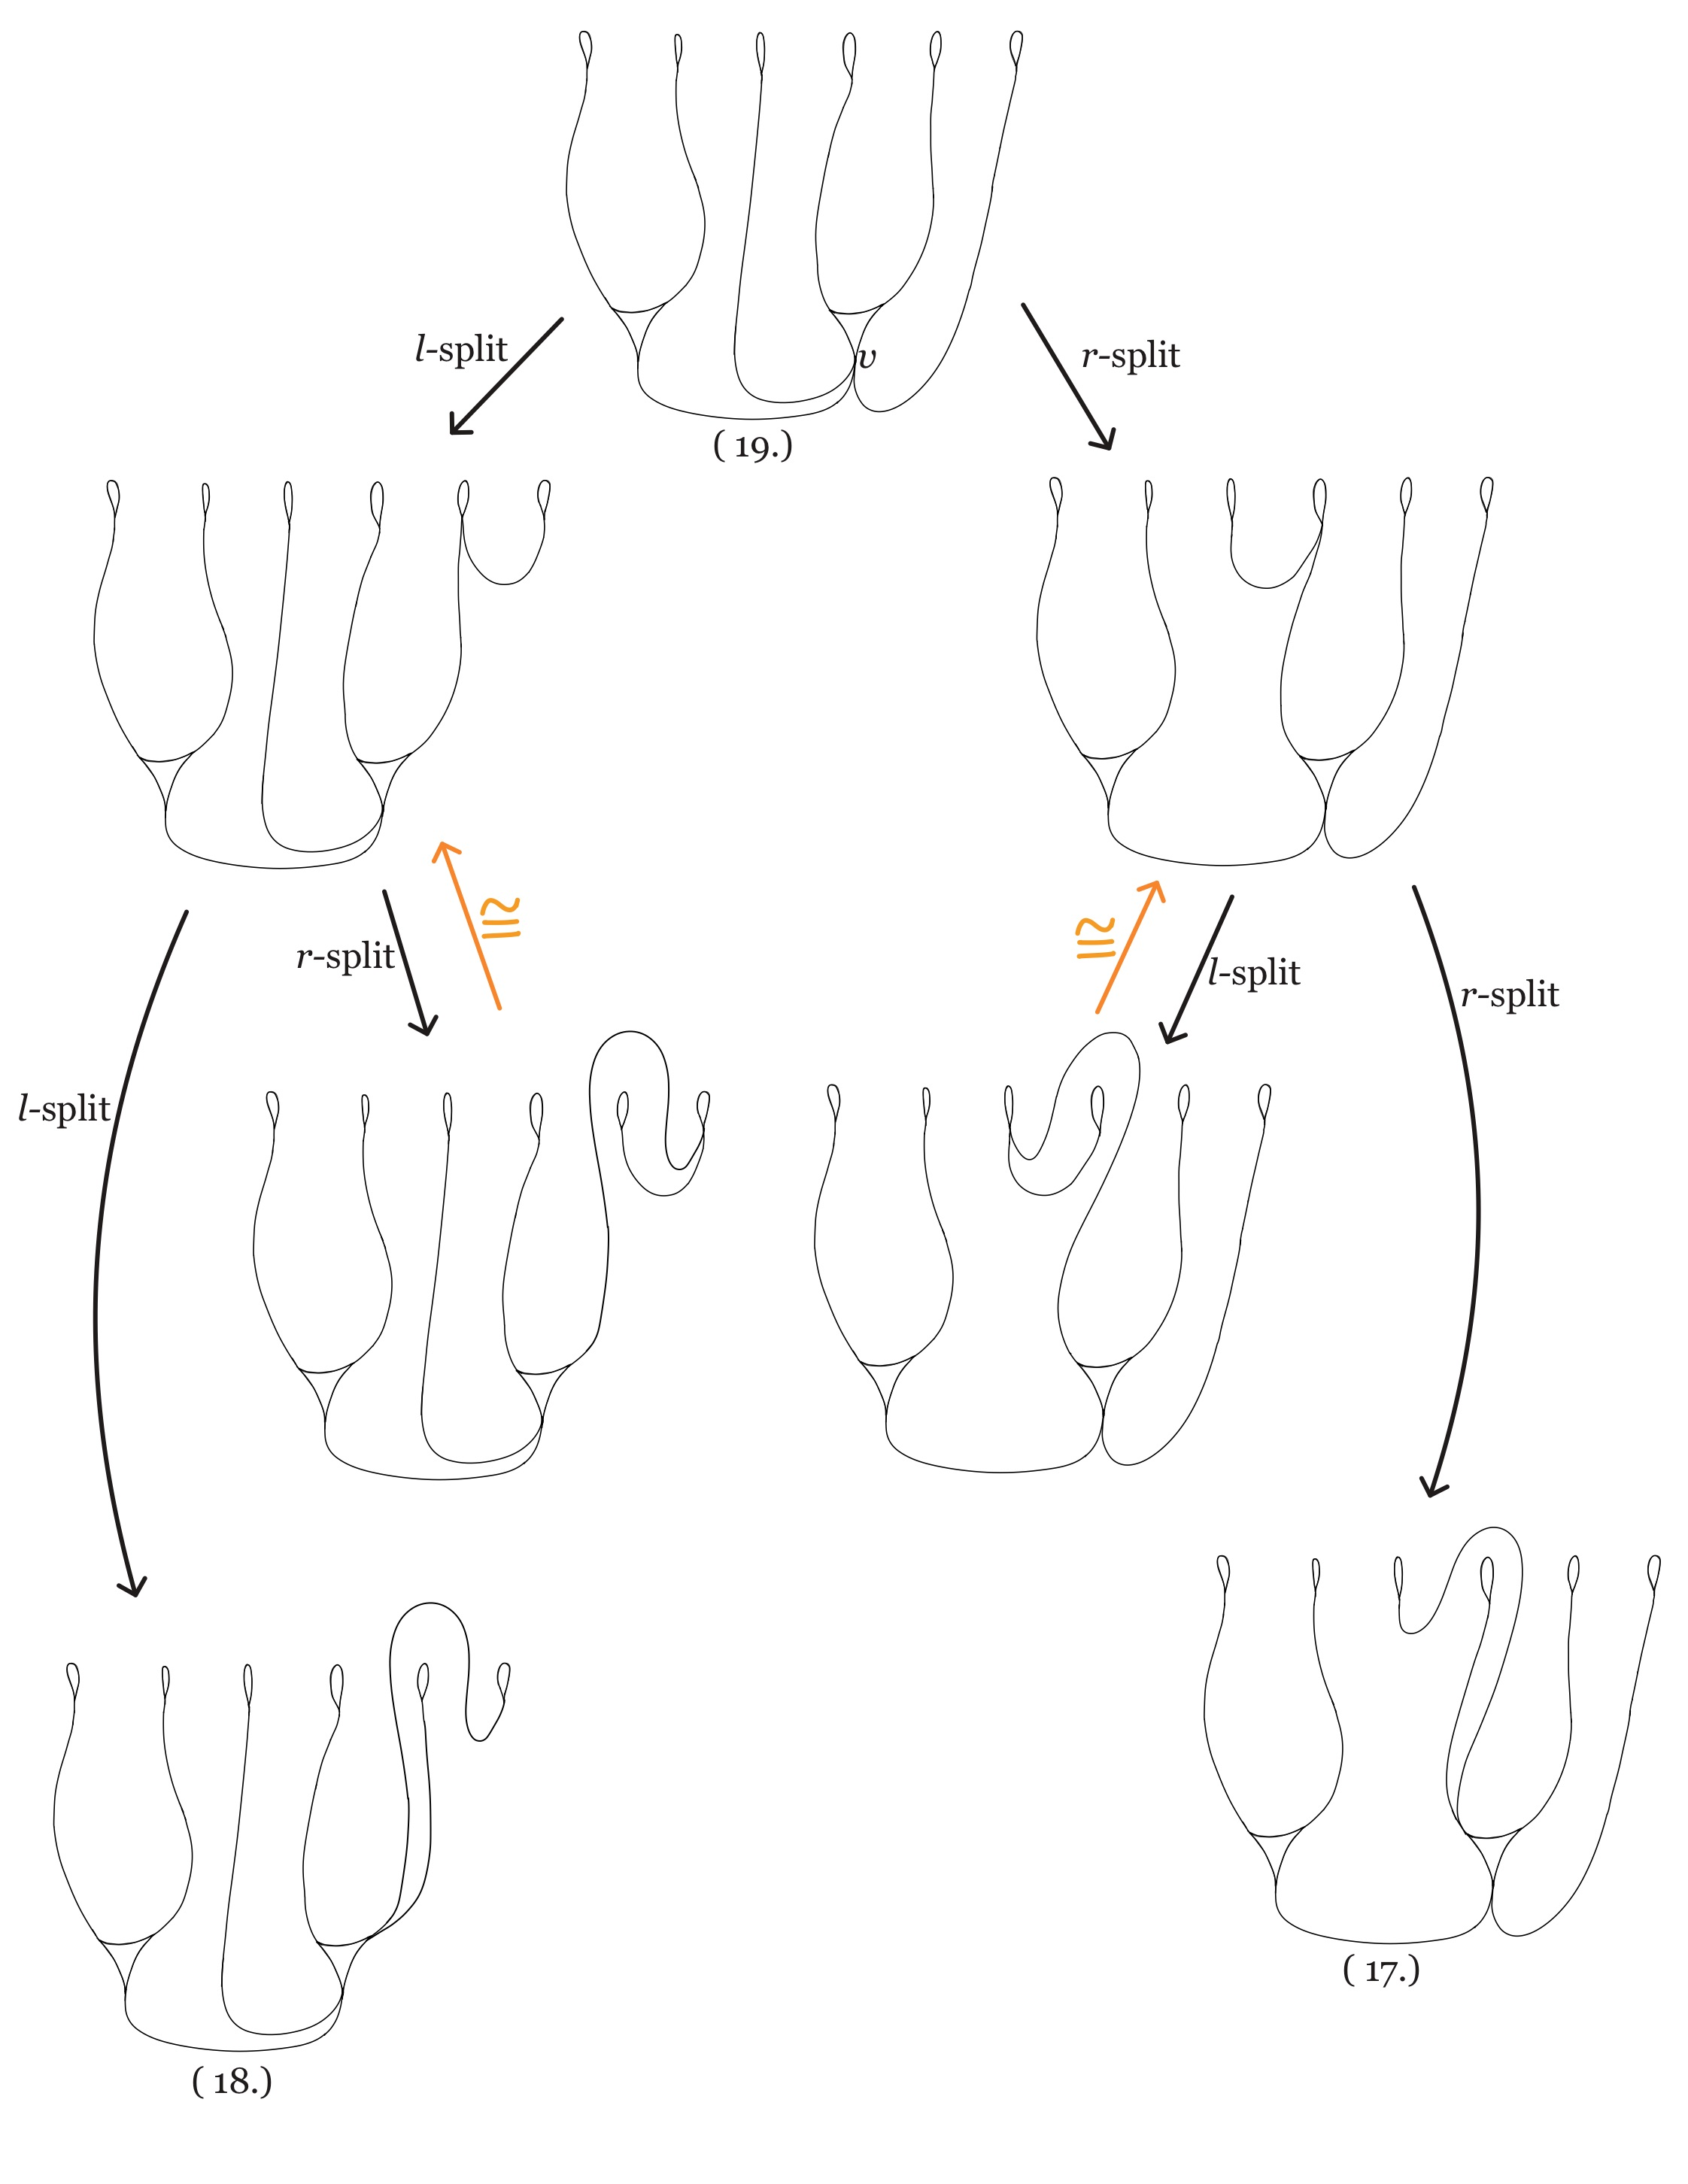
\includegraphics[width=\linewidth, height=0.45\textheight, keepaspectratio]{figures_splitting/19 Splitting-1.jpg}
    \caption{This splitting sequence shows train track (19.) eventually splits to the train tracks (18.) or (17.).} 
    \label{fig:19_splitting}
\end{figure*}

\begin{figure*}[p] % [p] forces this to be on its own page, which is often necessary for large figures
    \centering
    % Restrict height to 45% of the text block per image, maintaining aspect ratio
    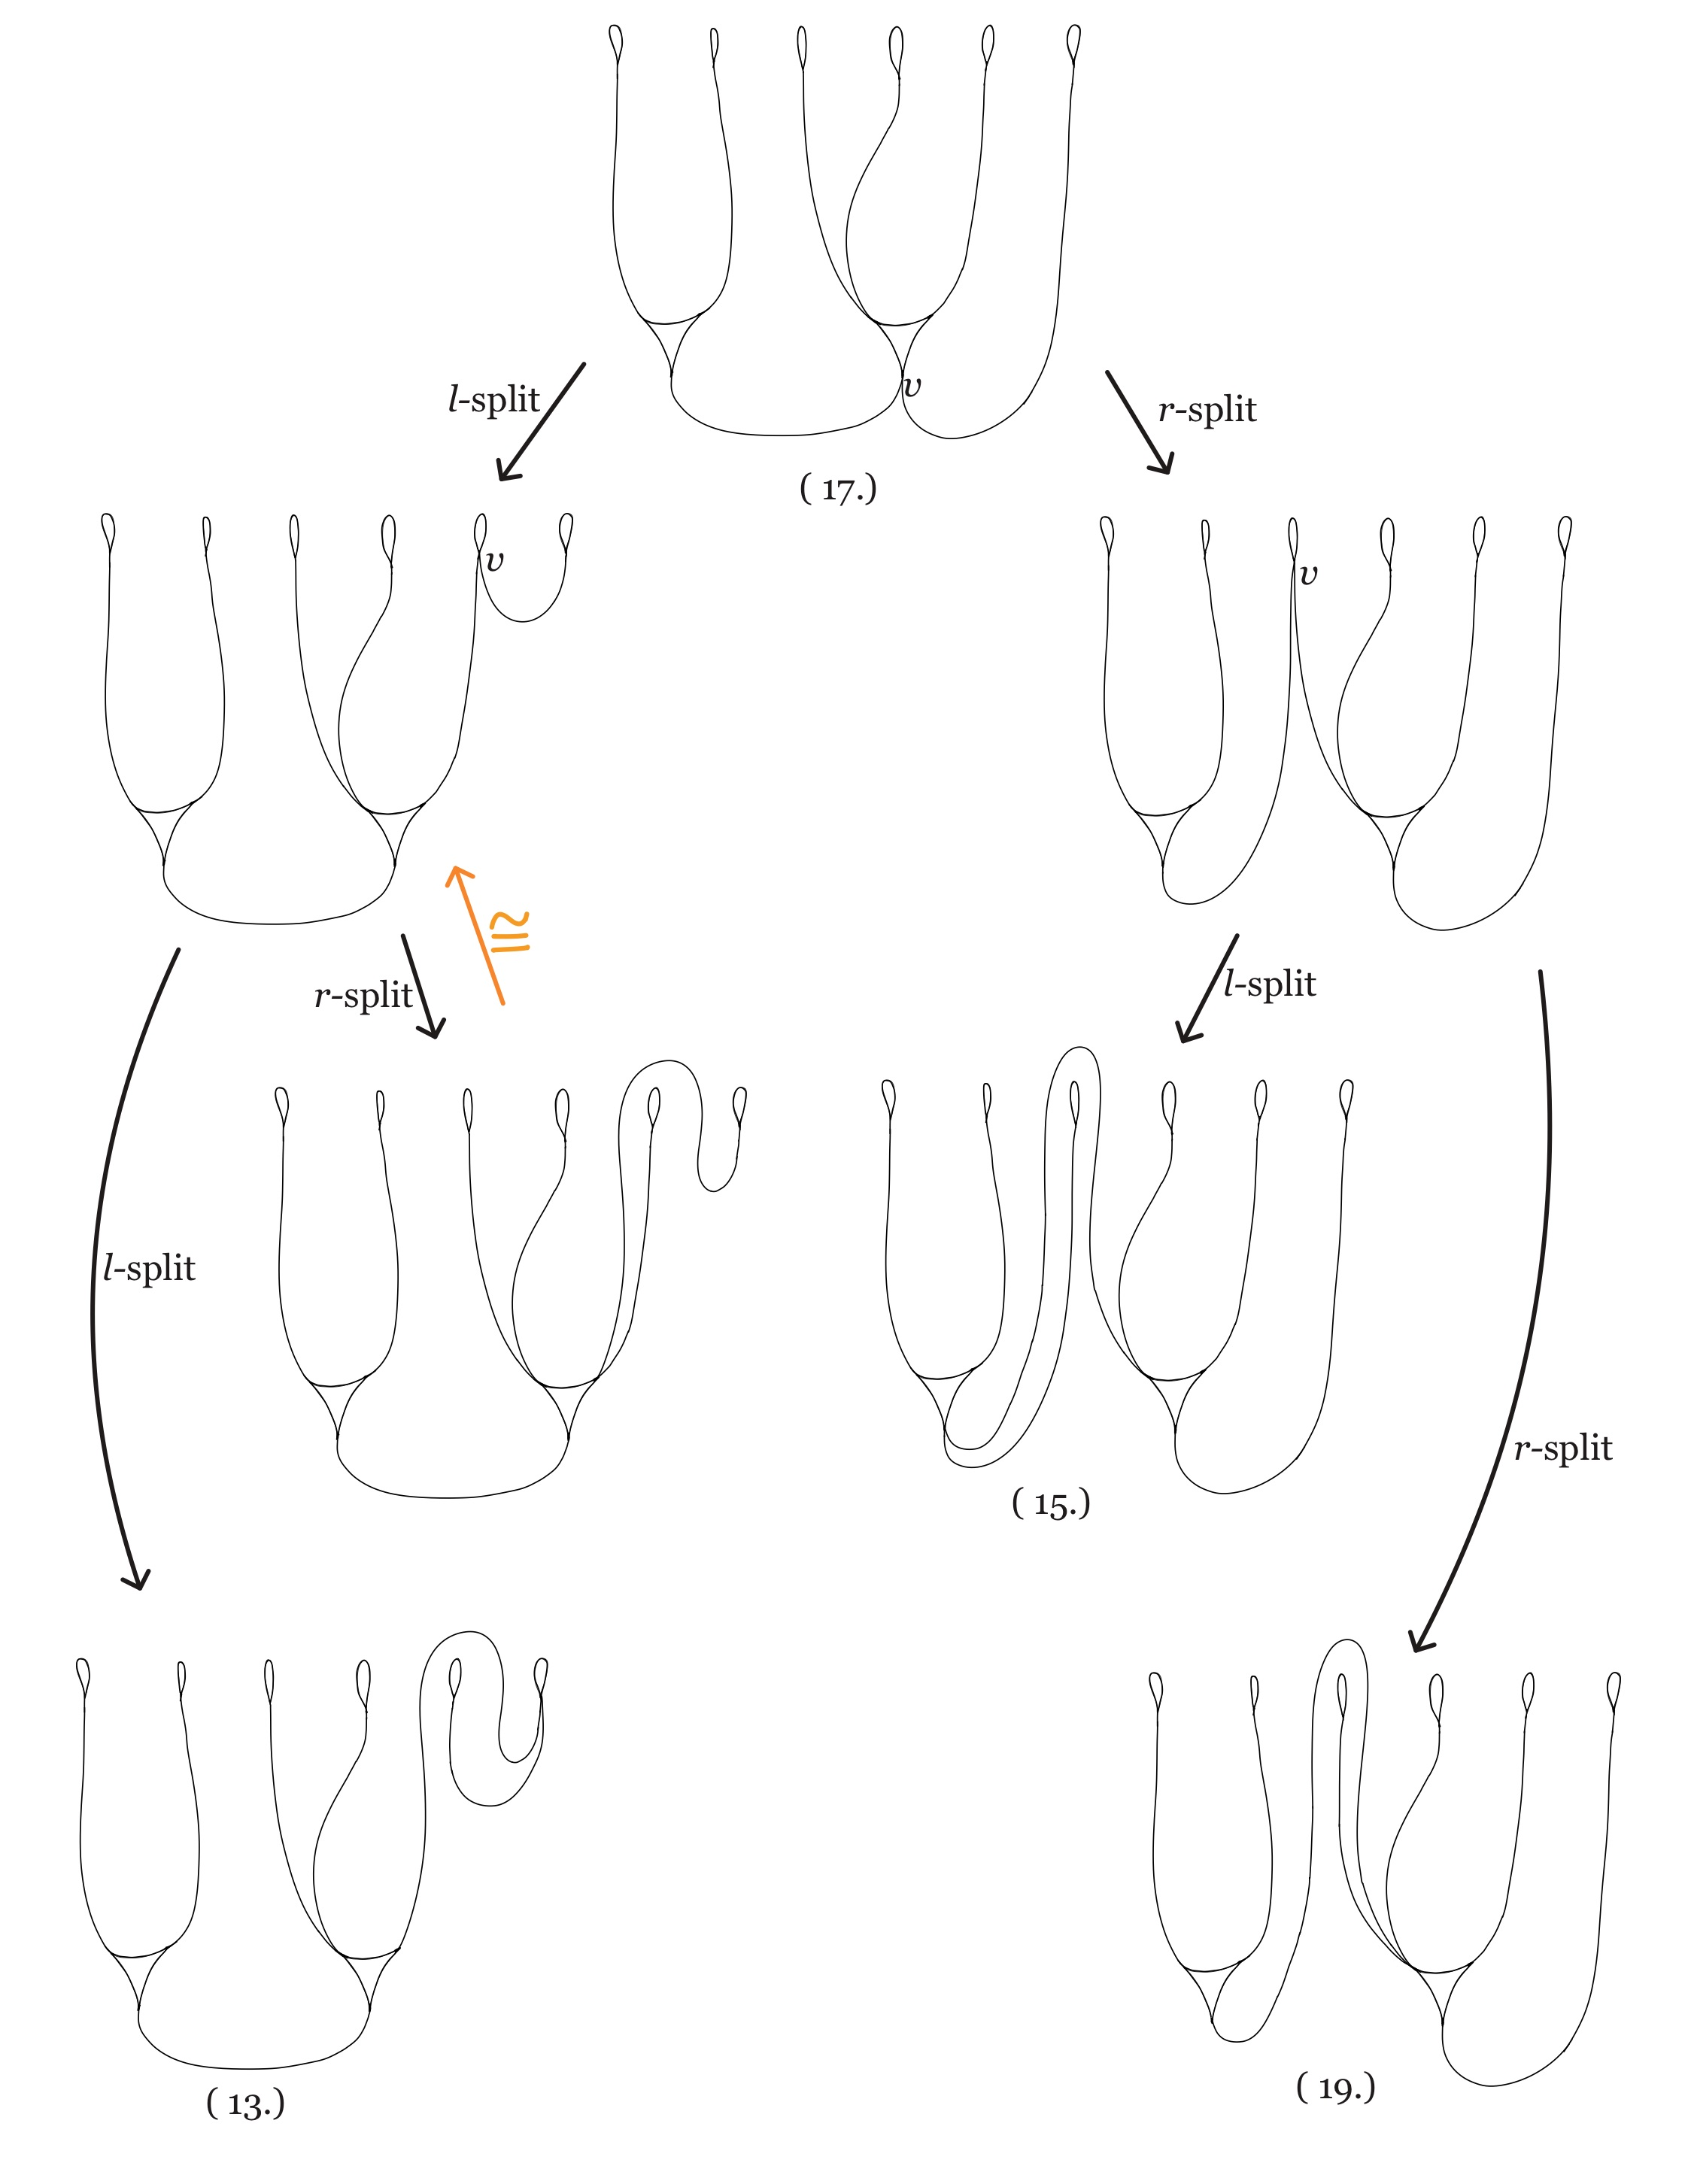
\includegraphics[width=\linewidth, height=0.45\textheight, keepaspectratio]{figures_splitting/17 Splitting-1.jpg}\\[0pt]
    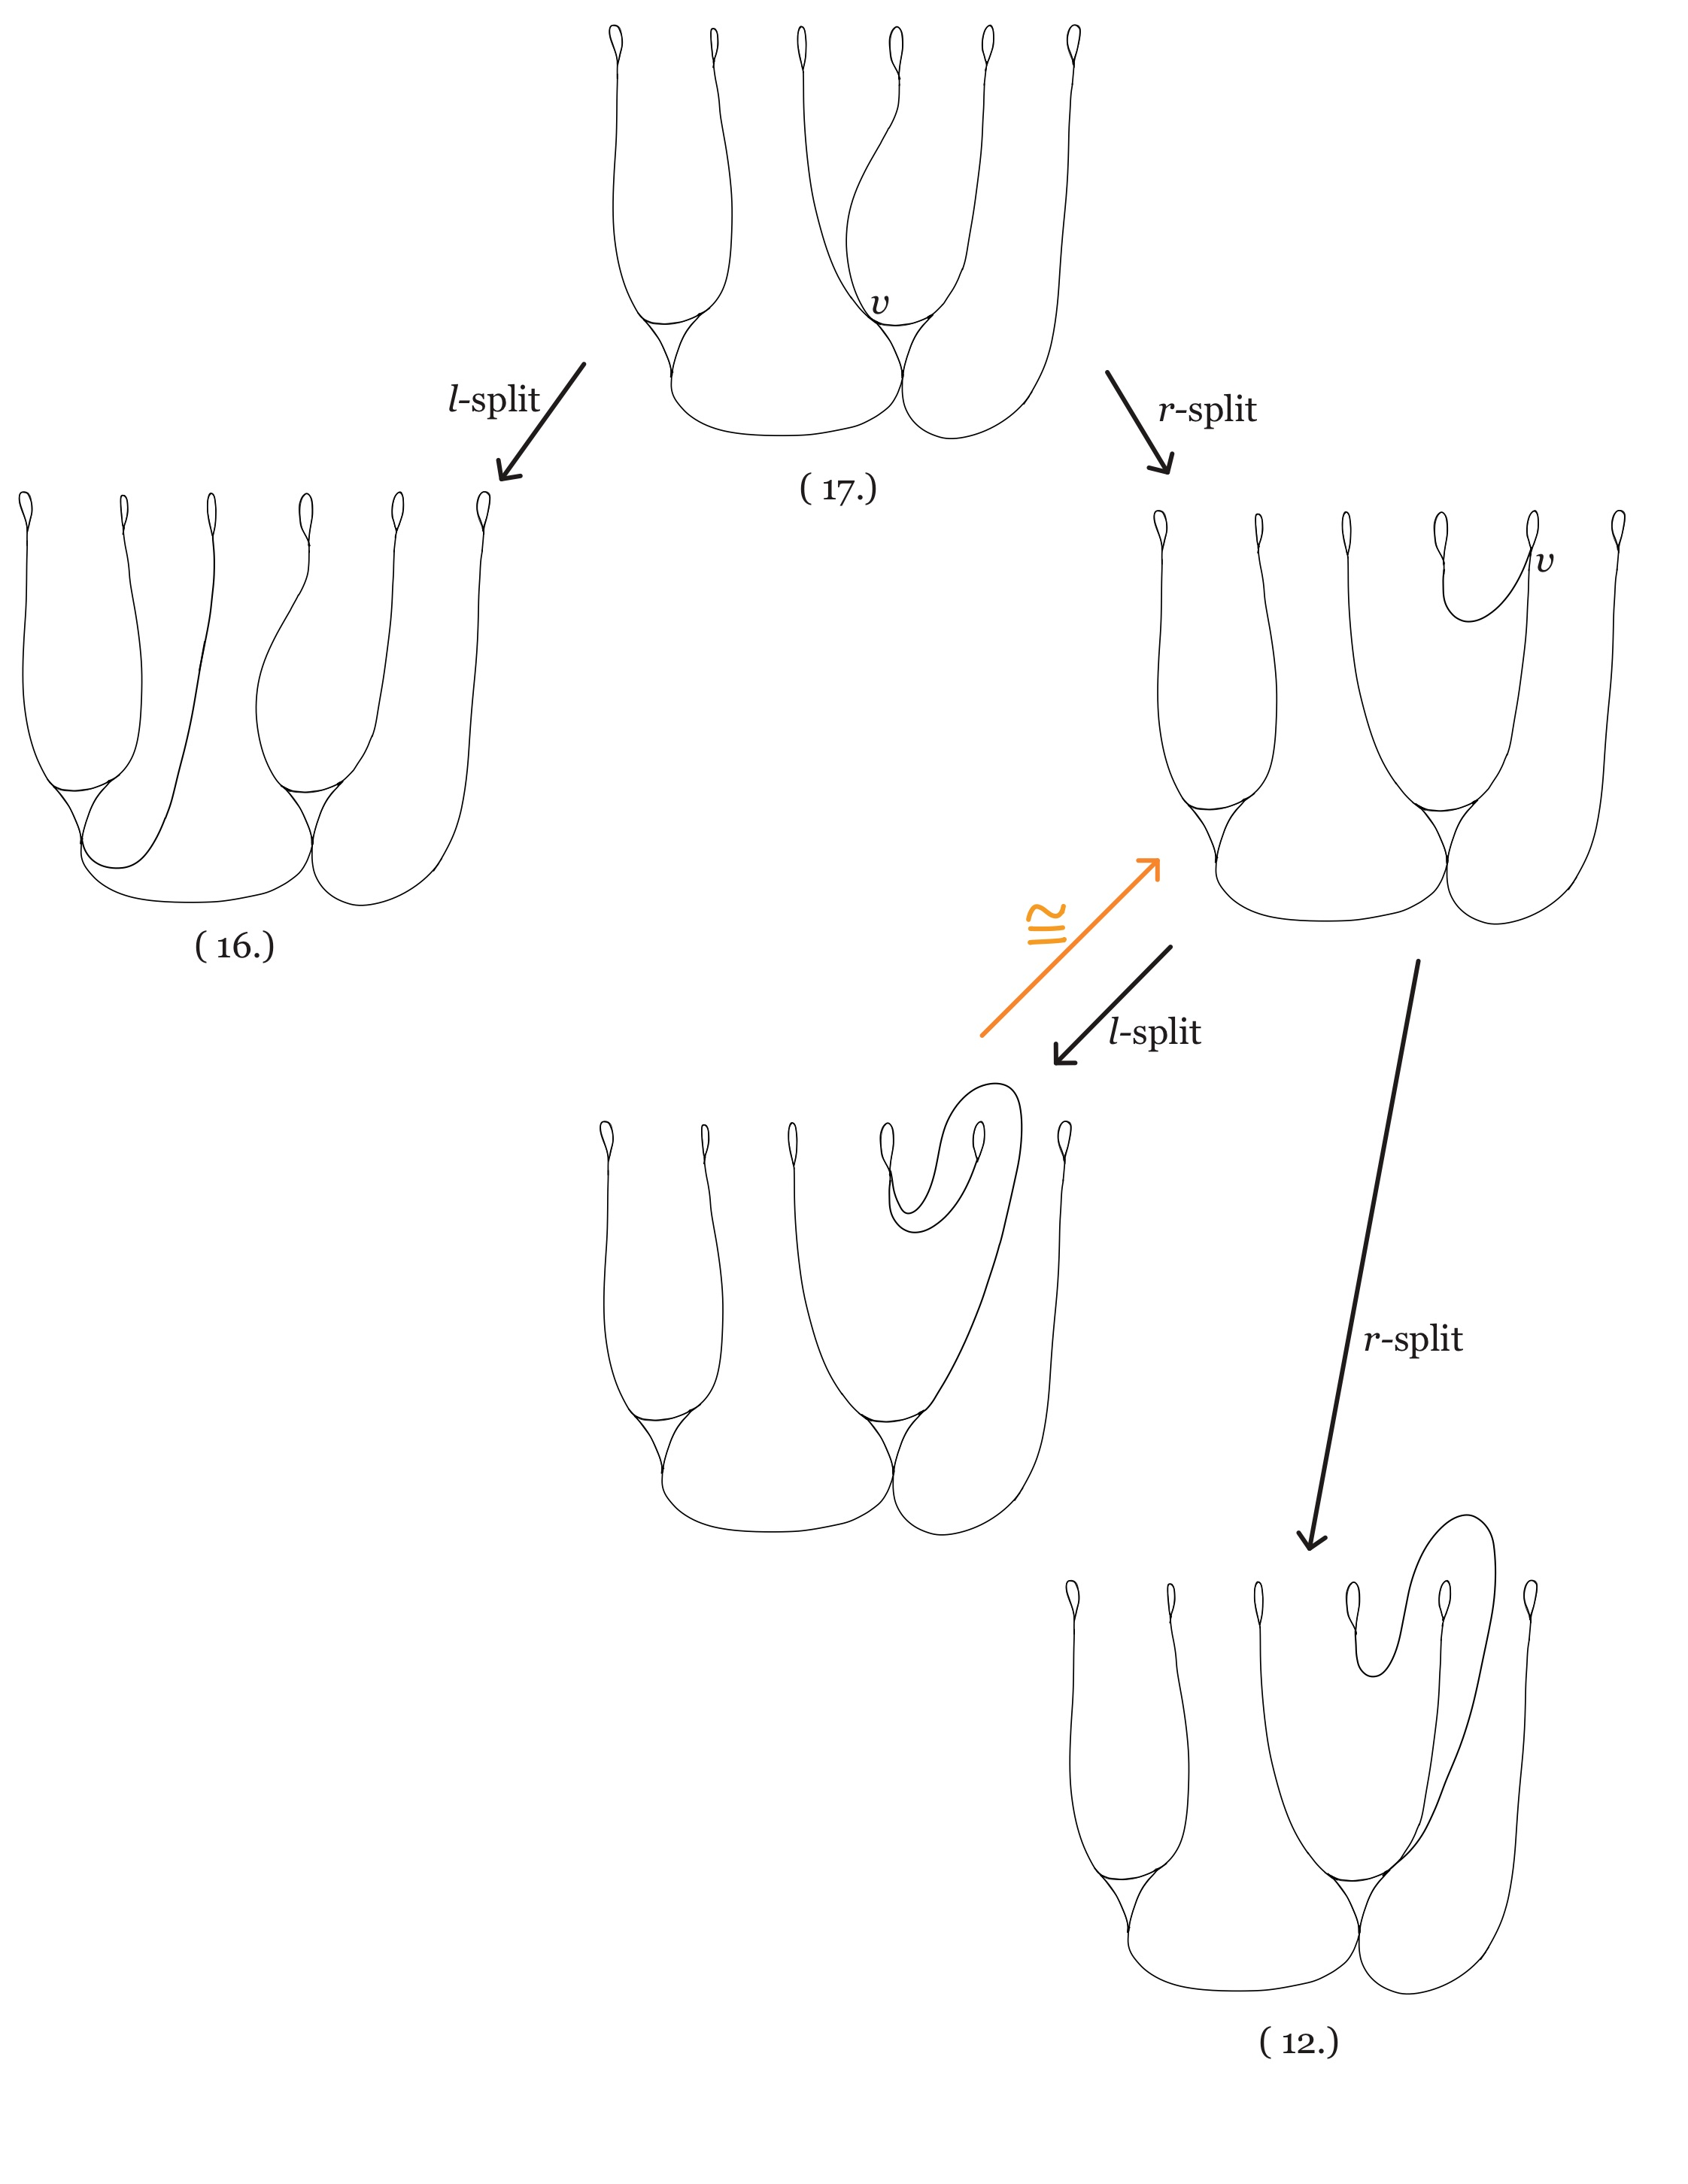
\includegraphics[width=\linewidth, height=0.45\textheight, keepaspectratio]{figures_splitting/17 Splitting-2.jpg}
    \caption{This splitting sequence shows train track (17.) eventually splits to the train tracks (19.), (13.), (16.), or (12.).}
    \label{fig:17_splitting}
\end{figure*}

\begin{figure*}[p] % [p] forces this to be on its own page, which is often necessary for large figures
    \centering
    % Restrict height to 45% of the text block per image, maintaining aspect ratio
    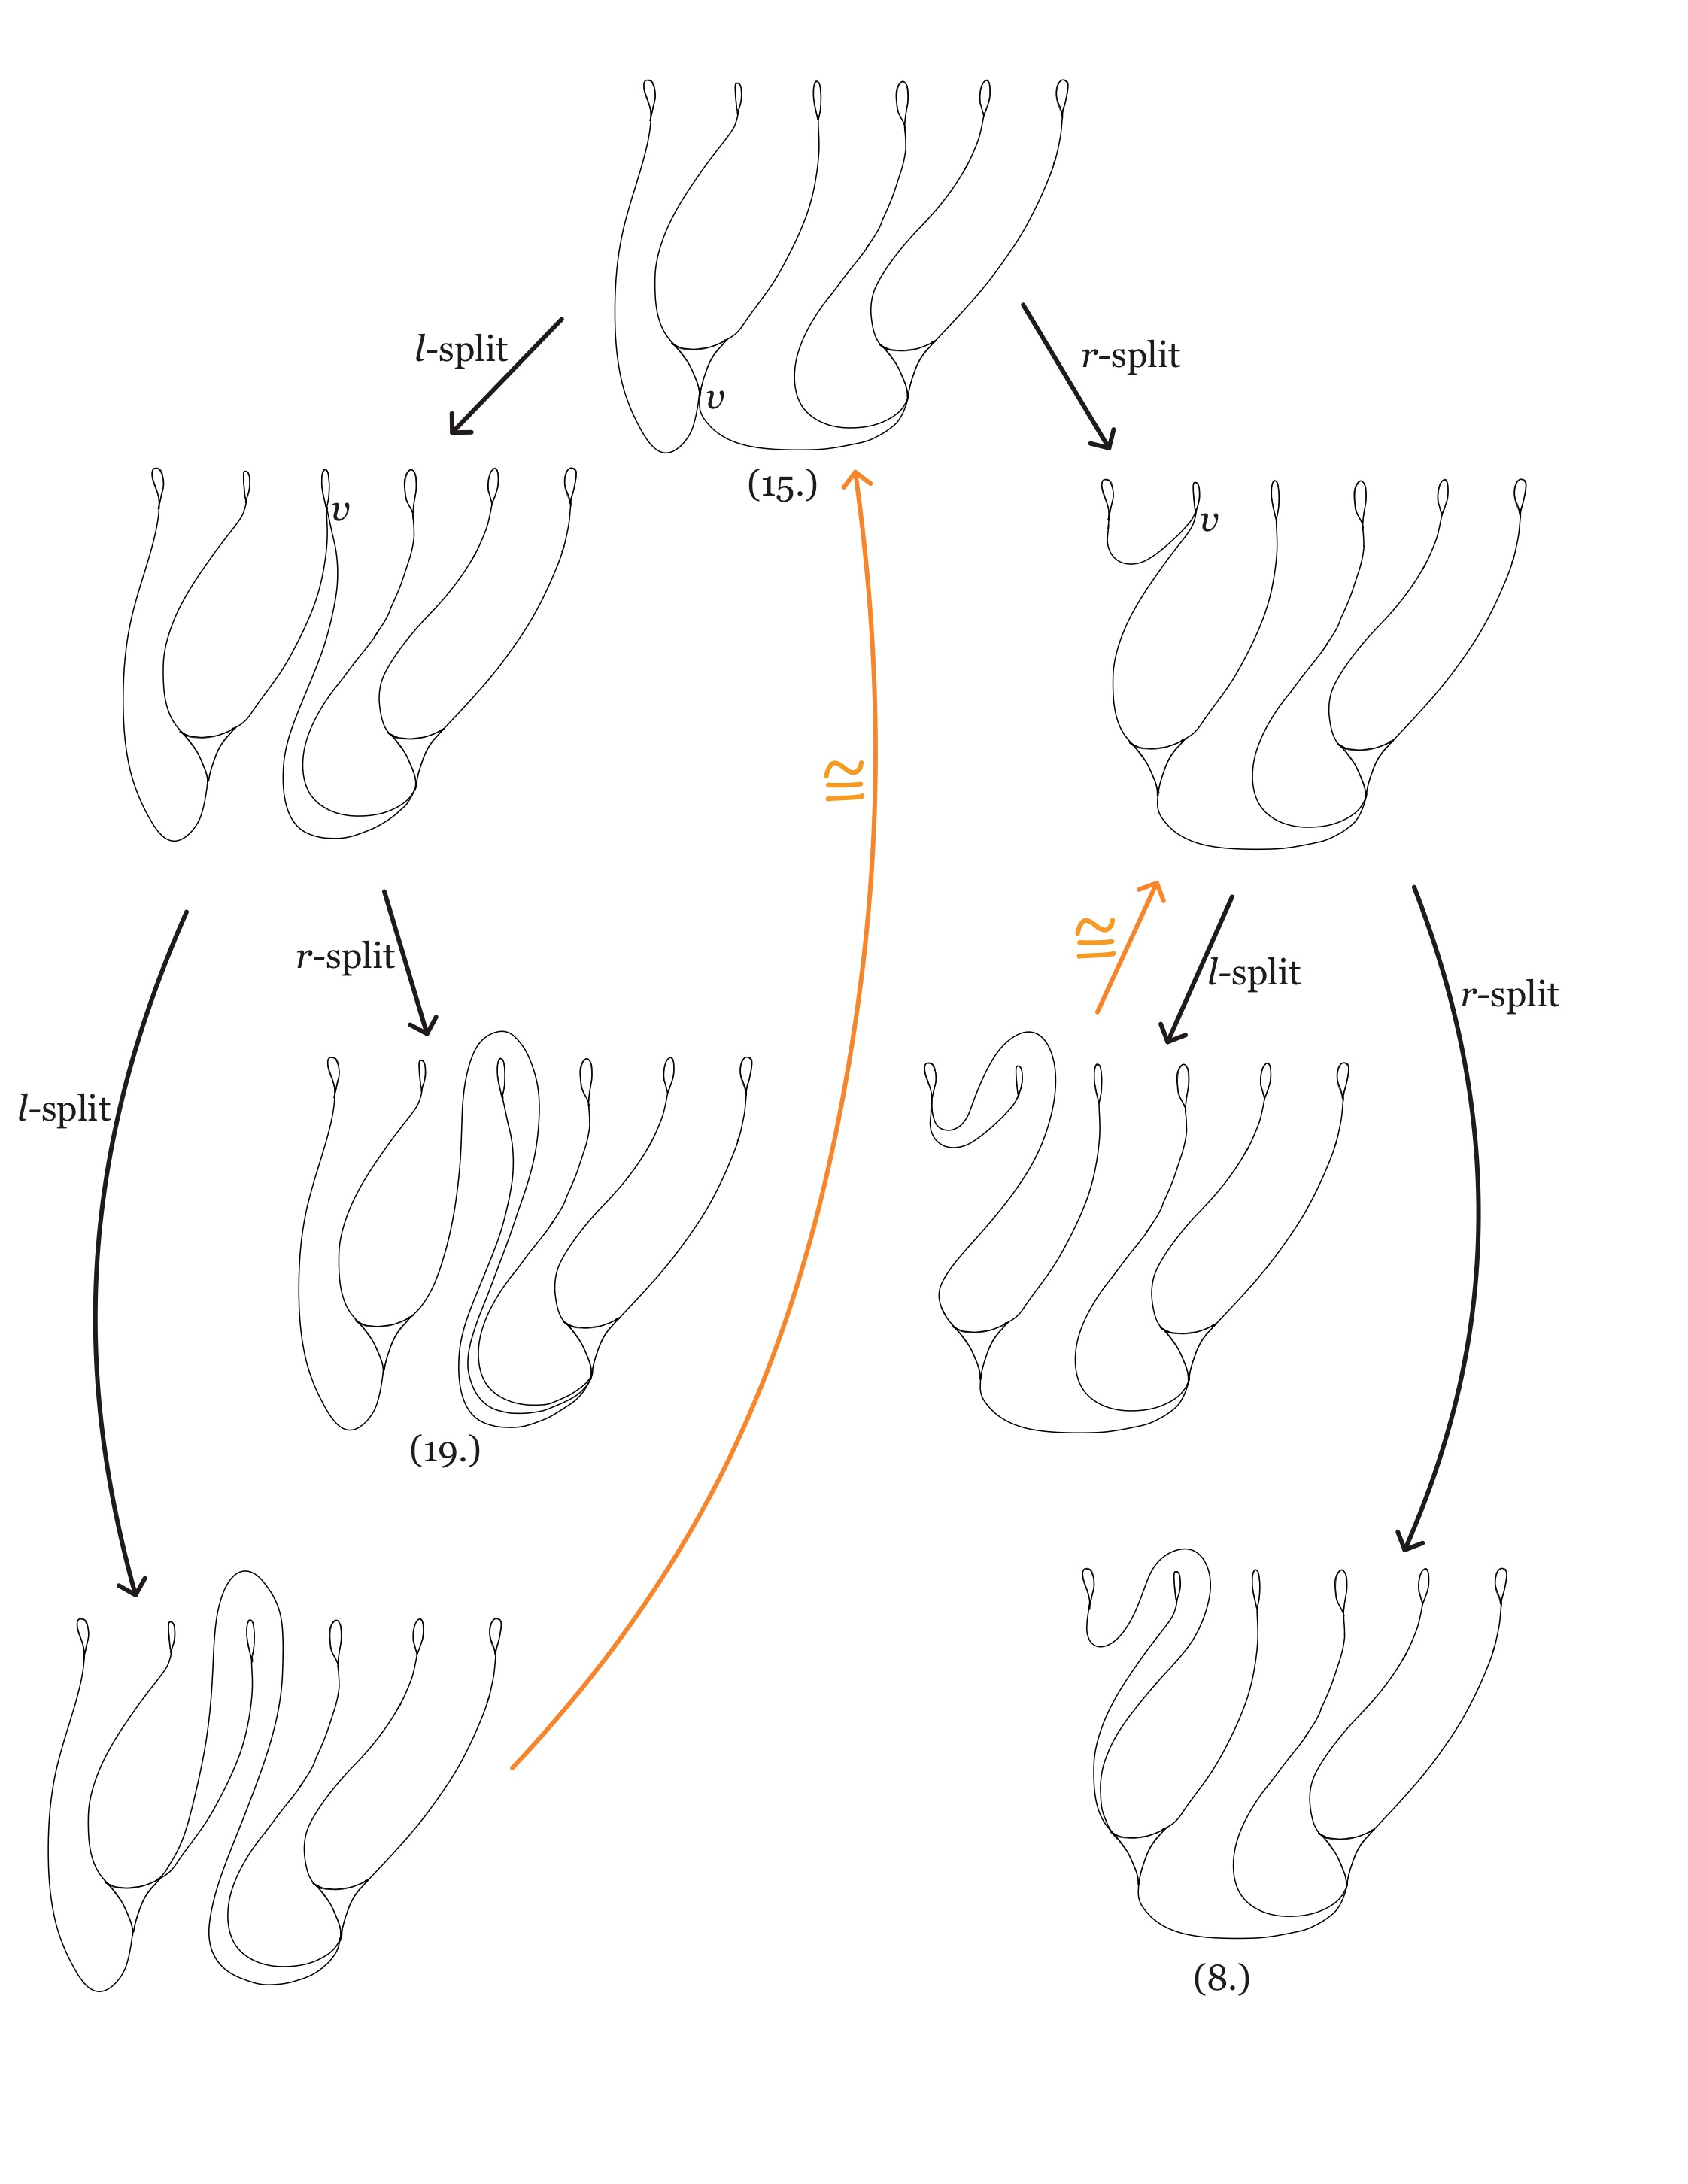
\includegraphics[width=\linewidth, height=0.45\textheight, keepaspectratio]{figures_splitting/15 Splitting-1.jpg}\\[0pt]
    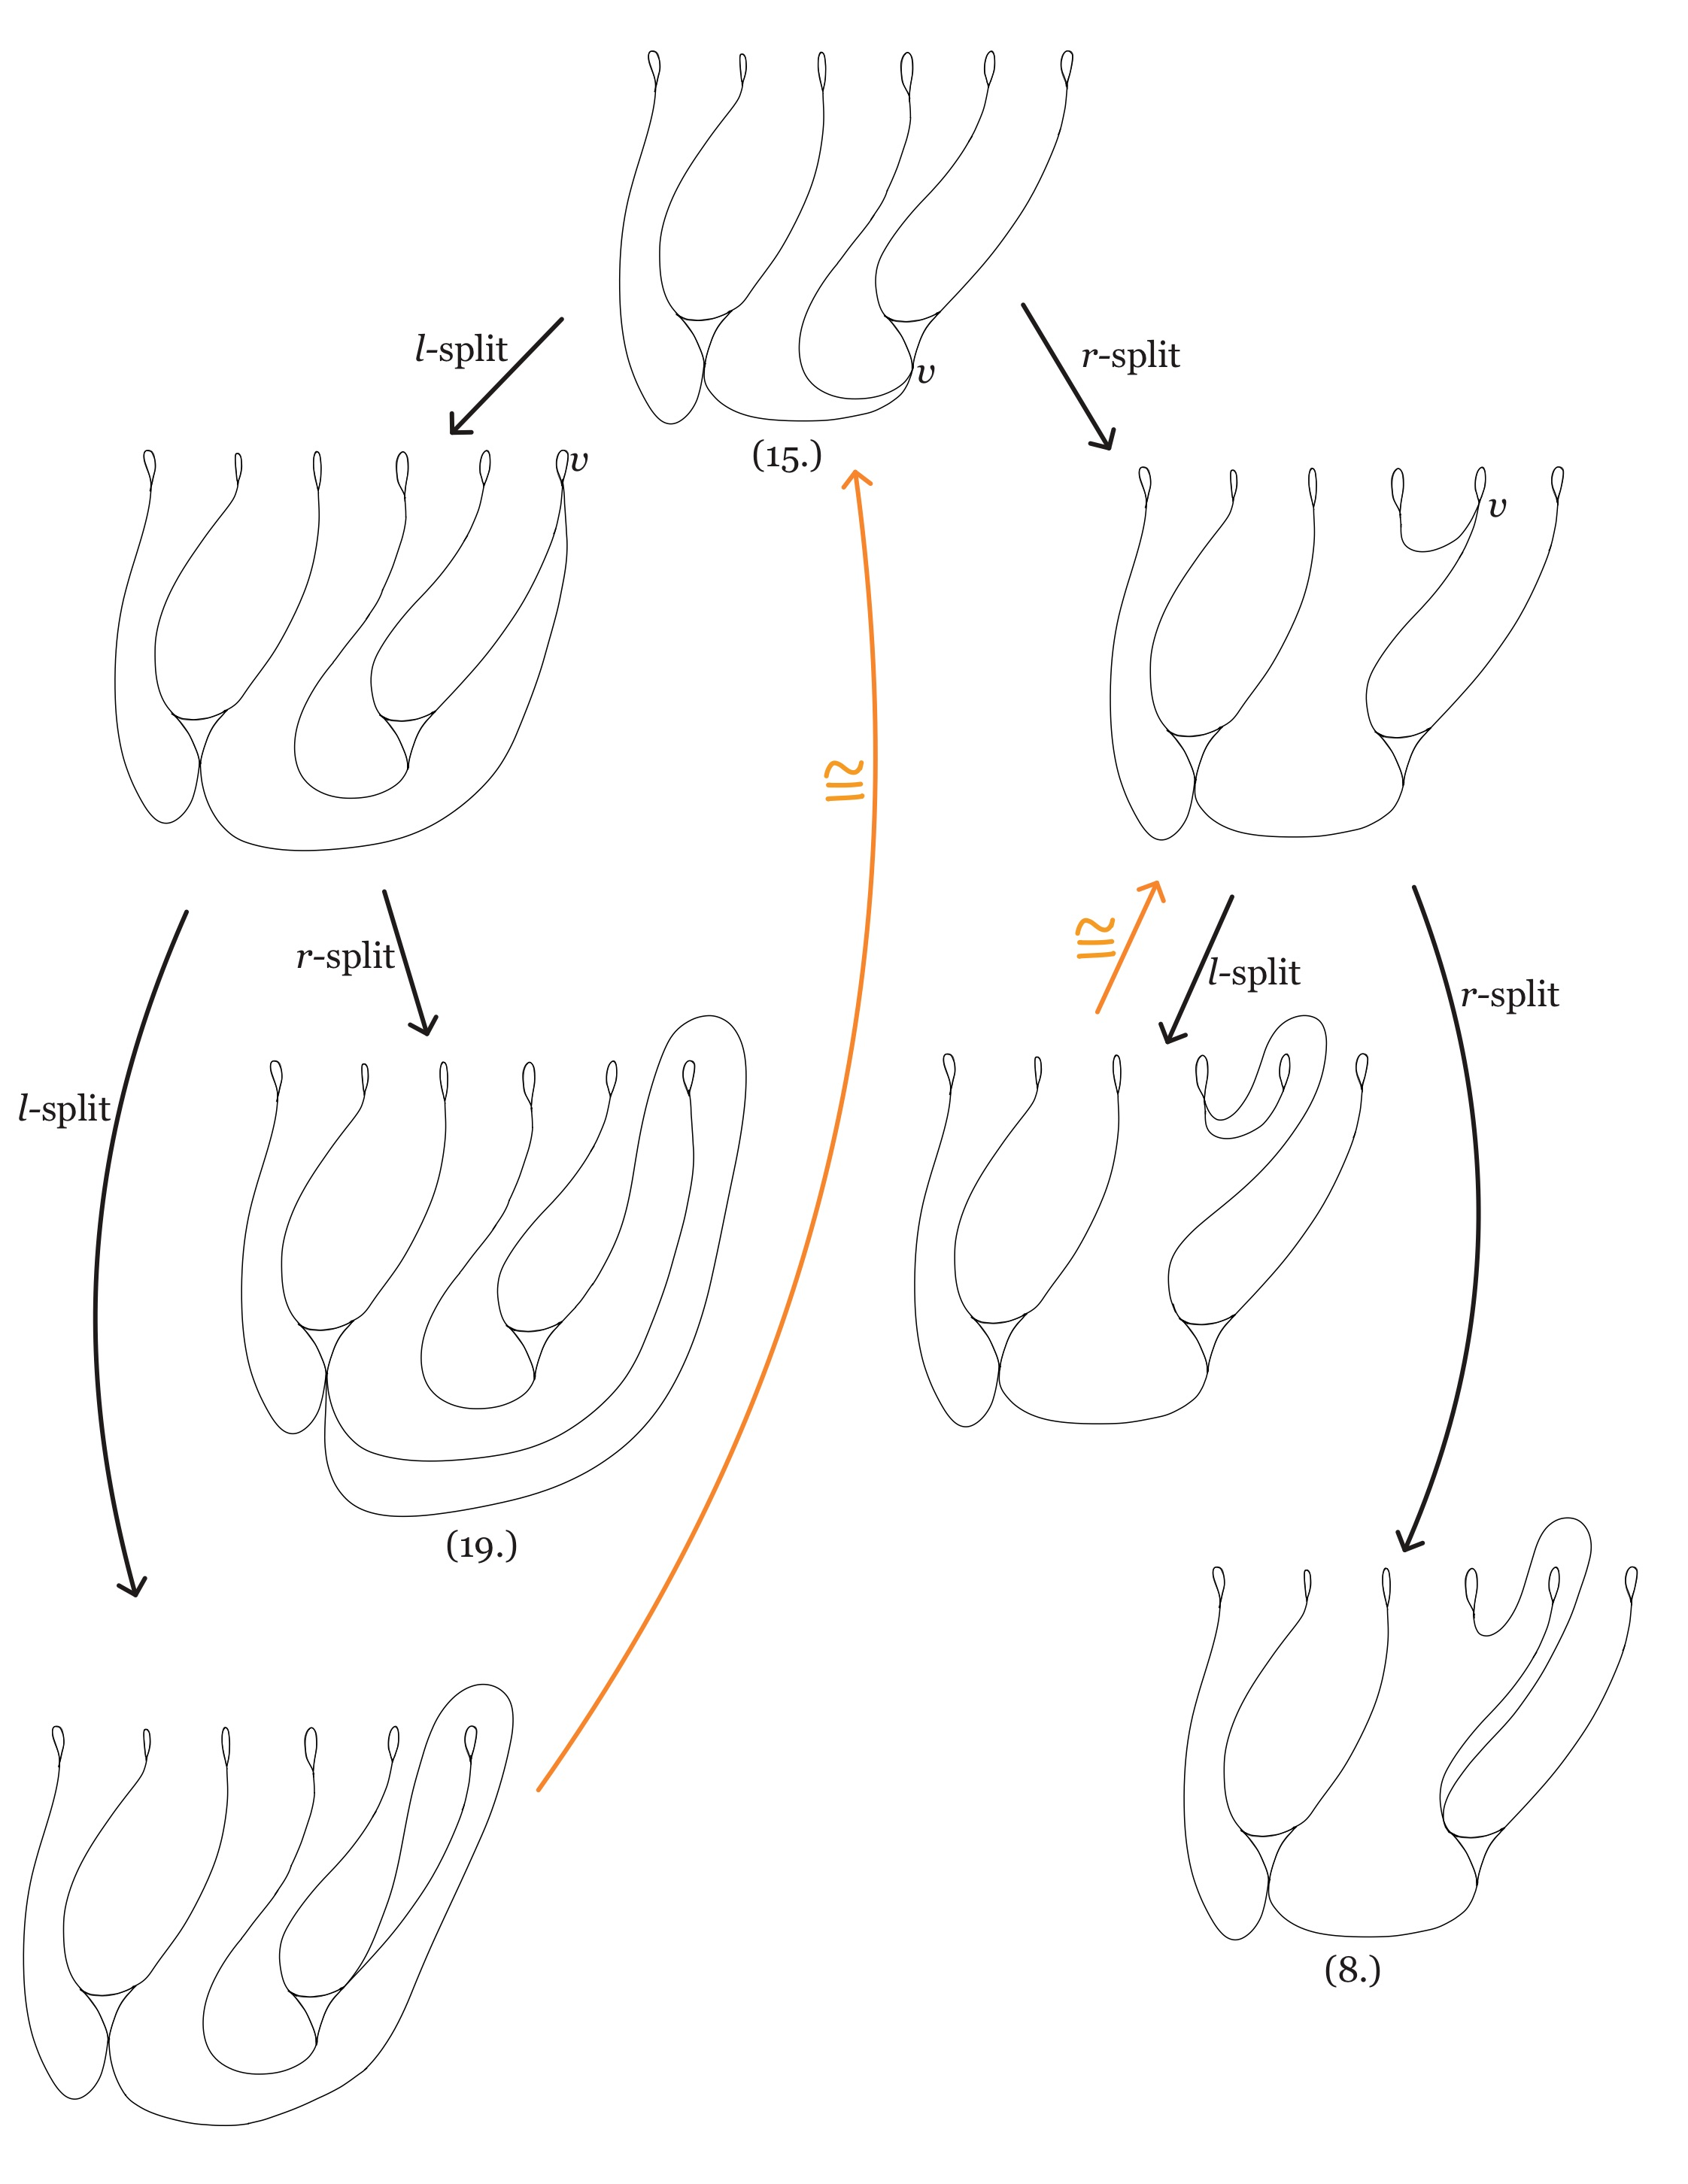
\includegraphics[width=\linewidth, height=0.45\textheight, keepaspectratio]{figures_splitting/15 Splitting-2.jpg}
    \caption{This splitting sequence shows train track (15.) eventually splits to the train tracks (19.) or (8.).}
    \label{fig:c15_splitting}
\end{figure*}

\begin{figure*}[p] % [p] forces this to be on its own page, which is often necessary for large figures
    \centering
    % Restrict height to 45% of the text block per image, maintaining aspect ratio
    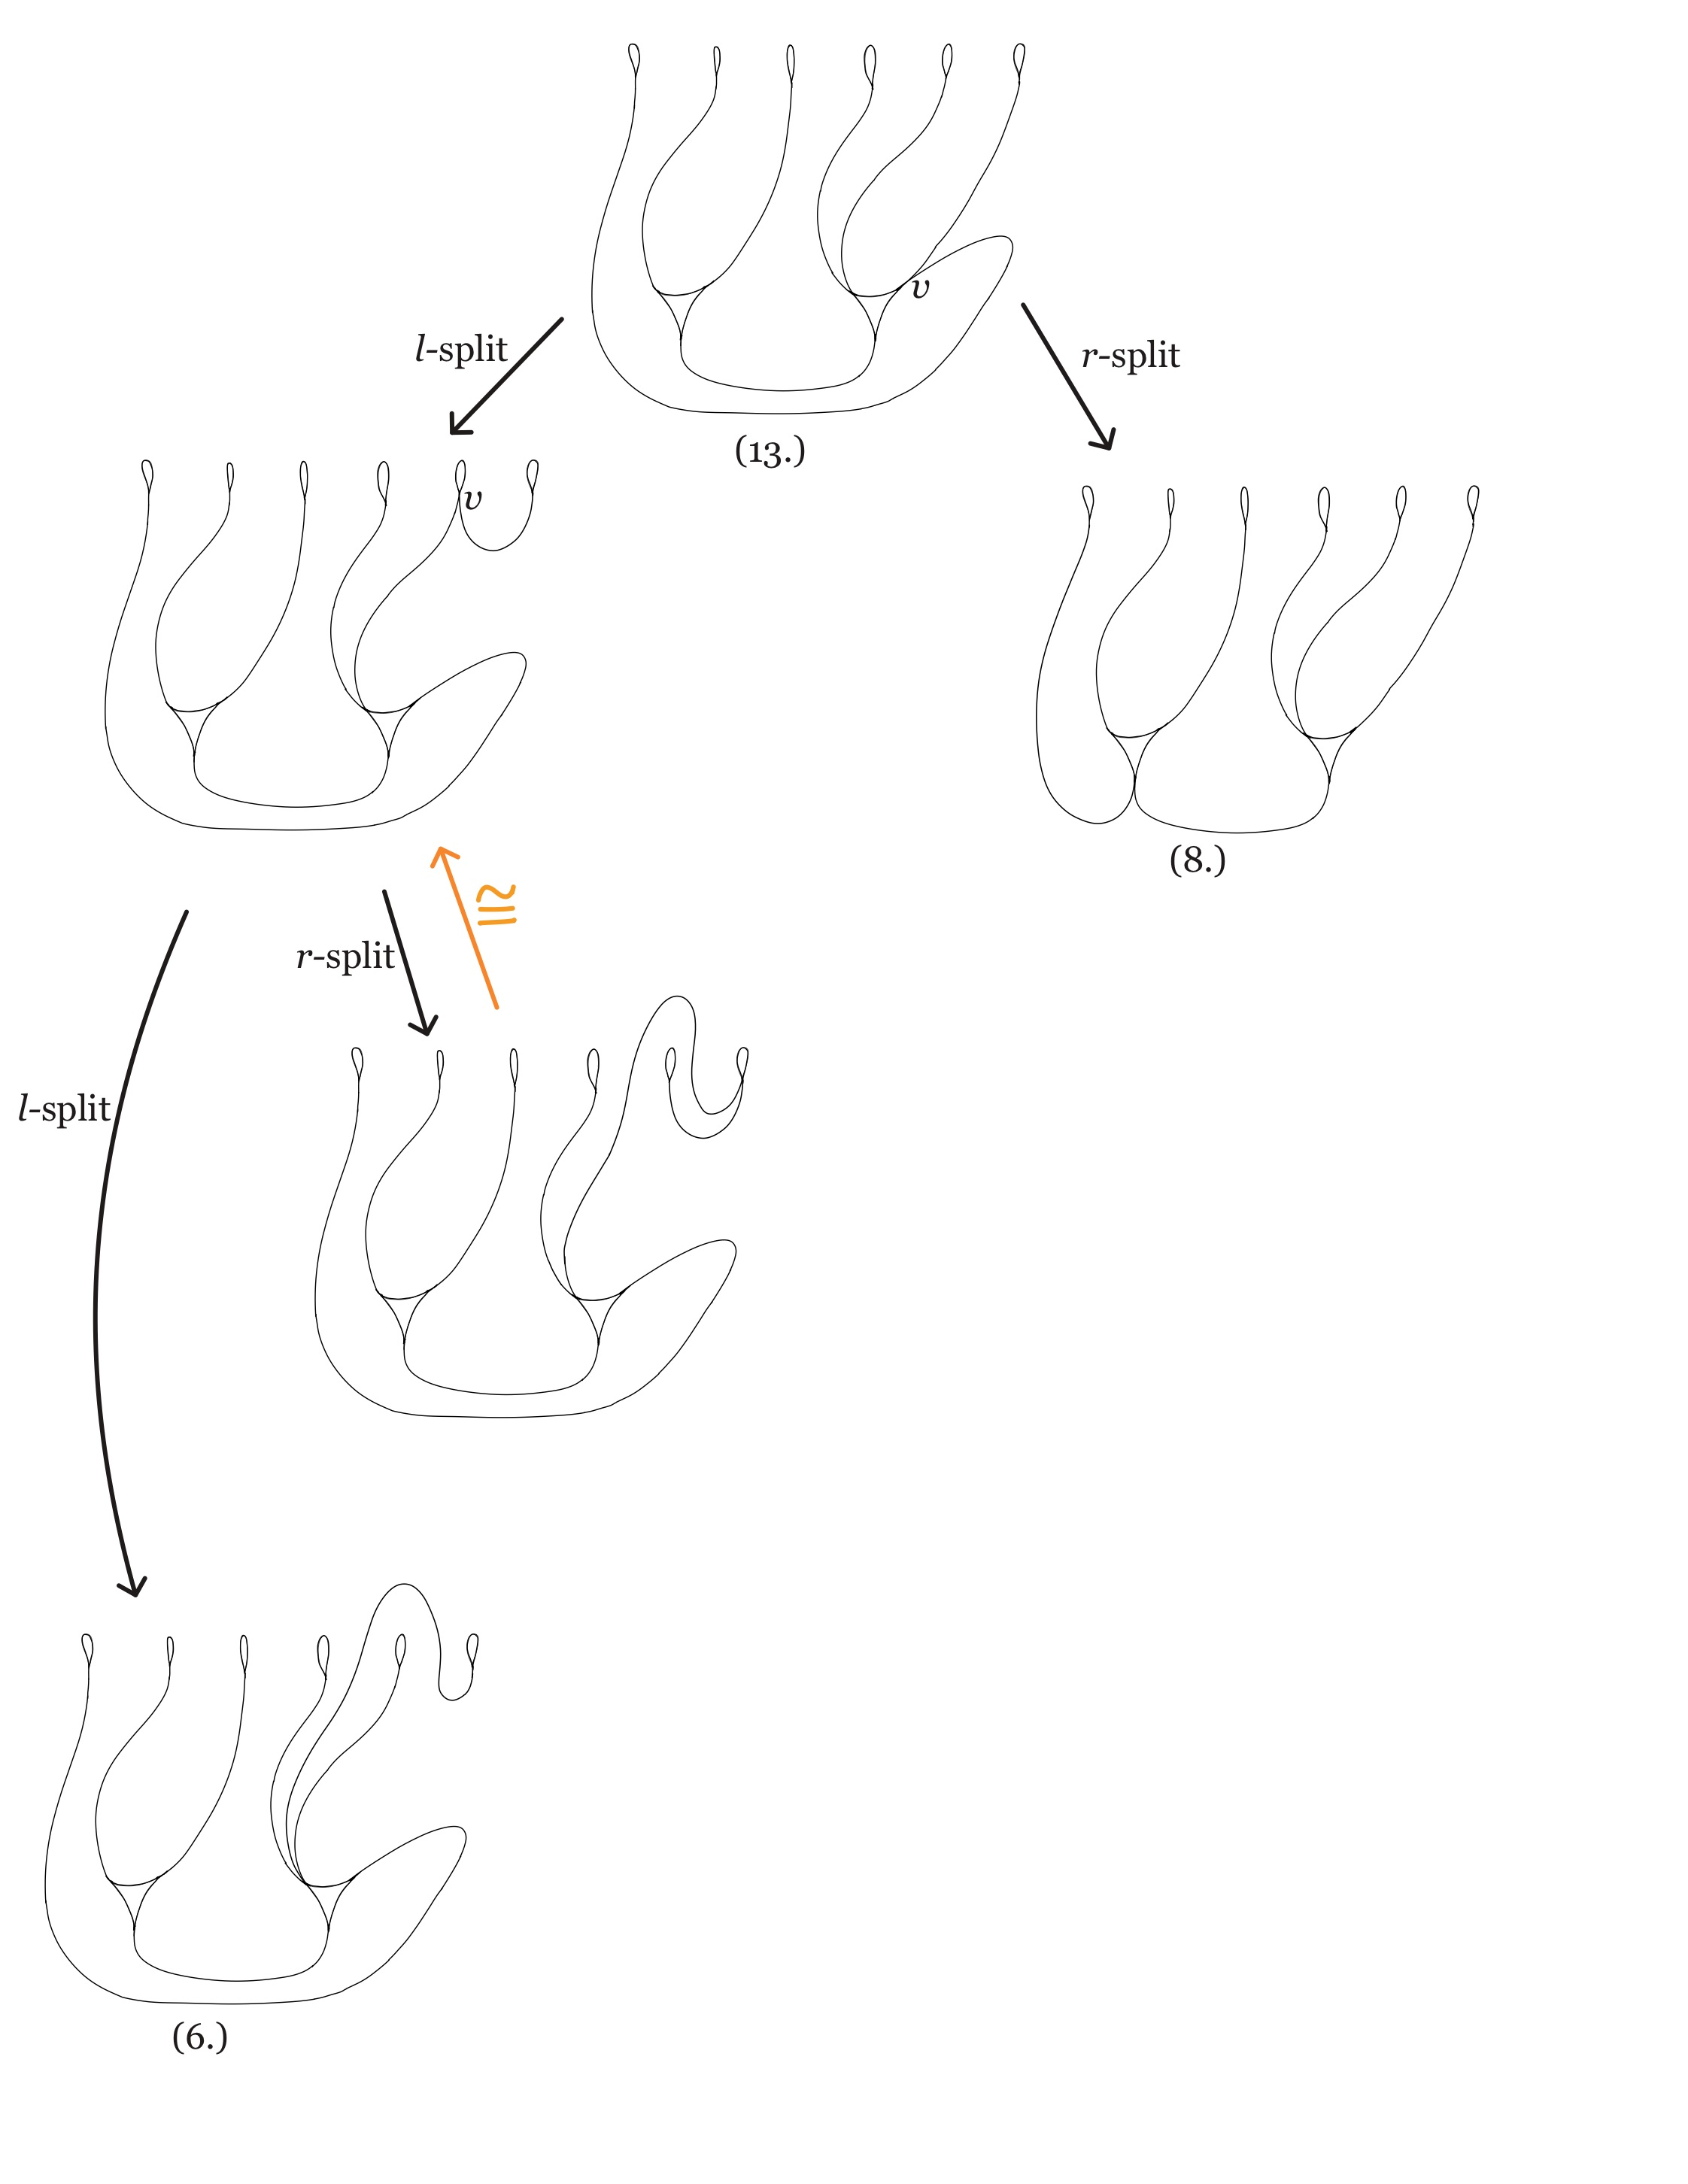
\includegraphics[width=\linewidth, height=0.45\textheight, keepaspectratio]{figures_splitting/13 Splitting-1.jpg}\\[0pt]
    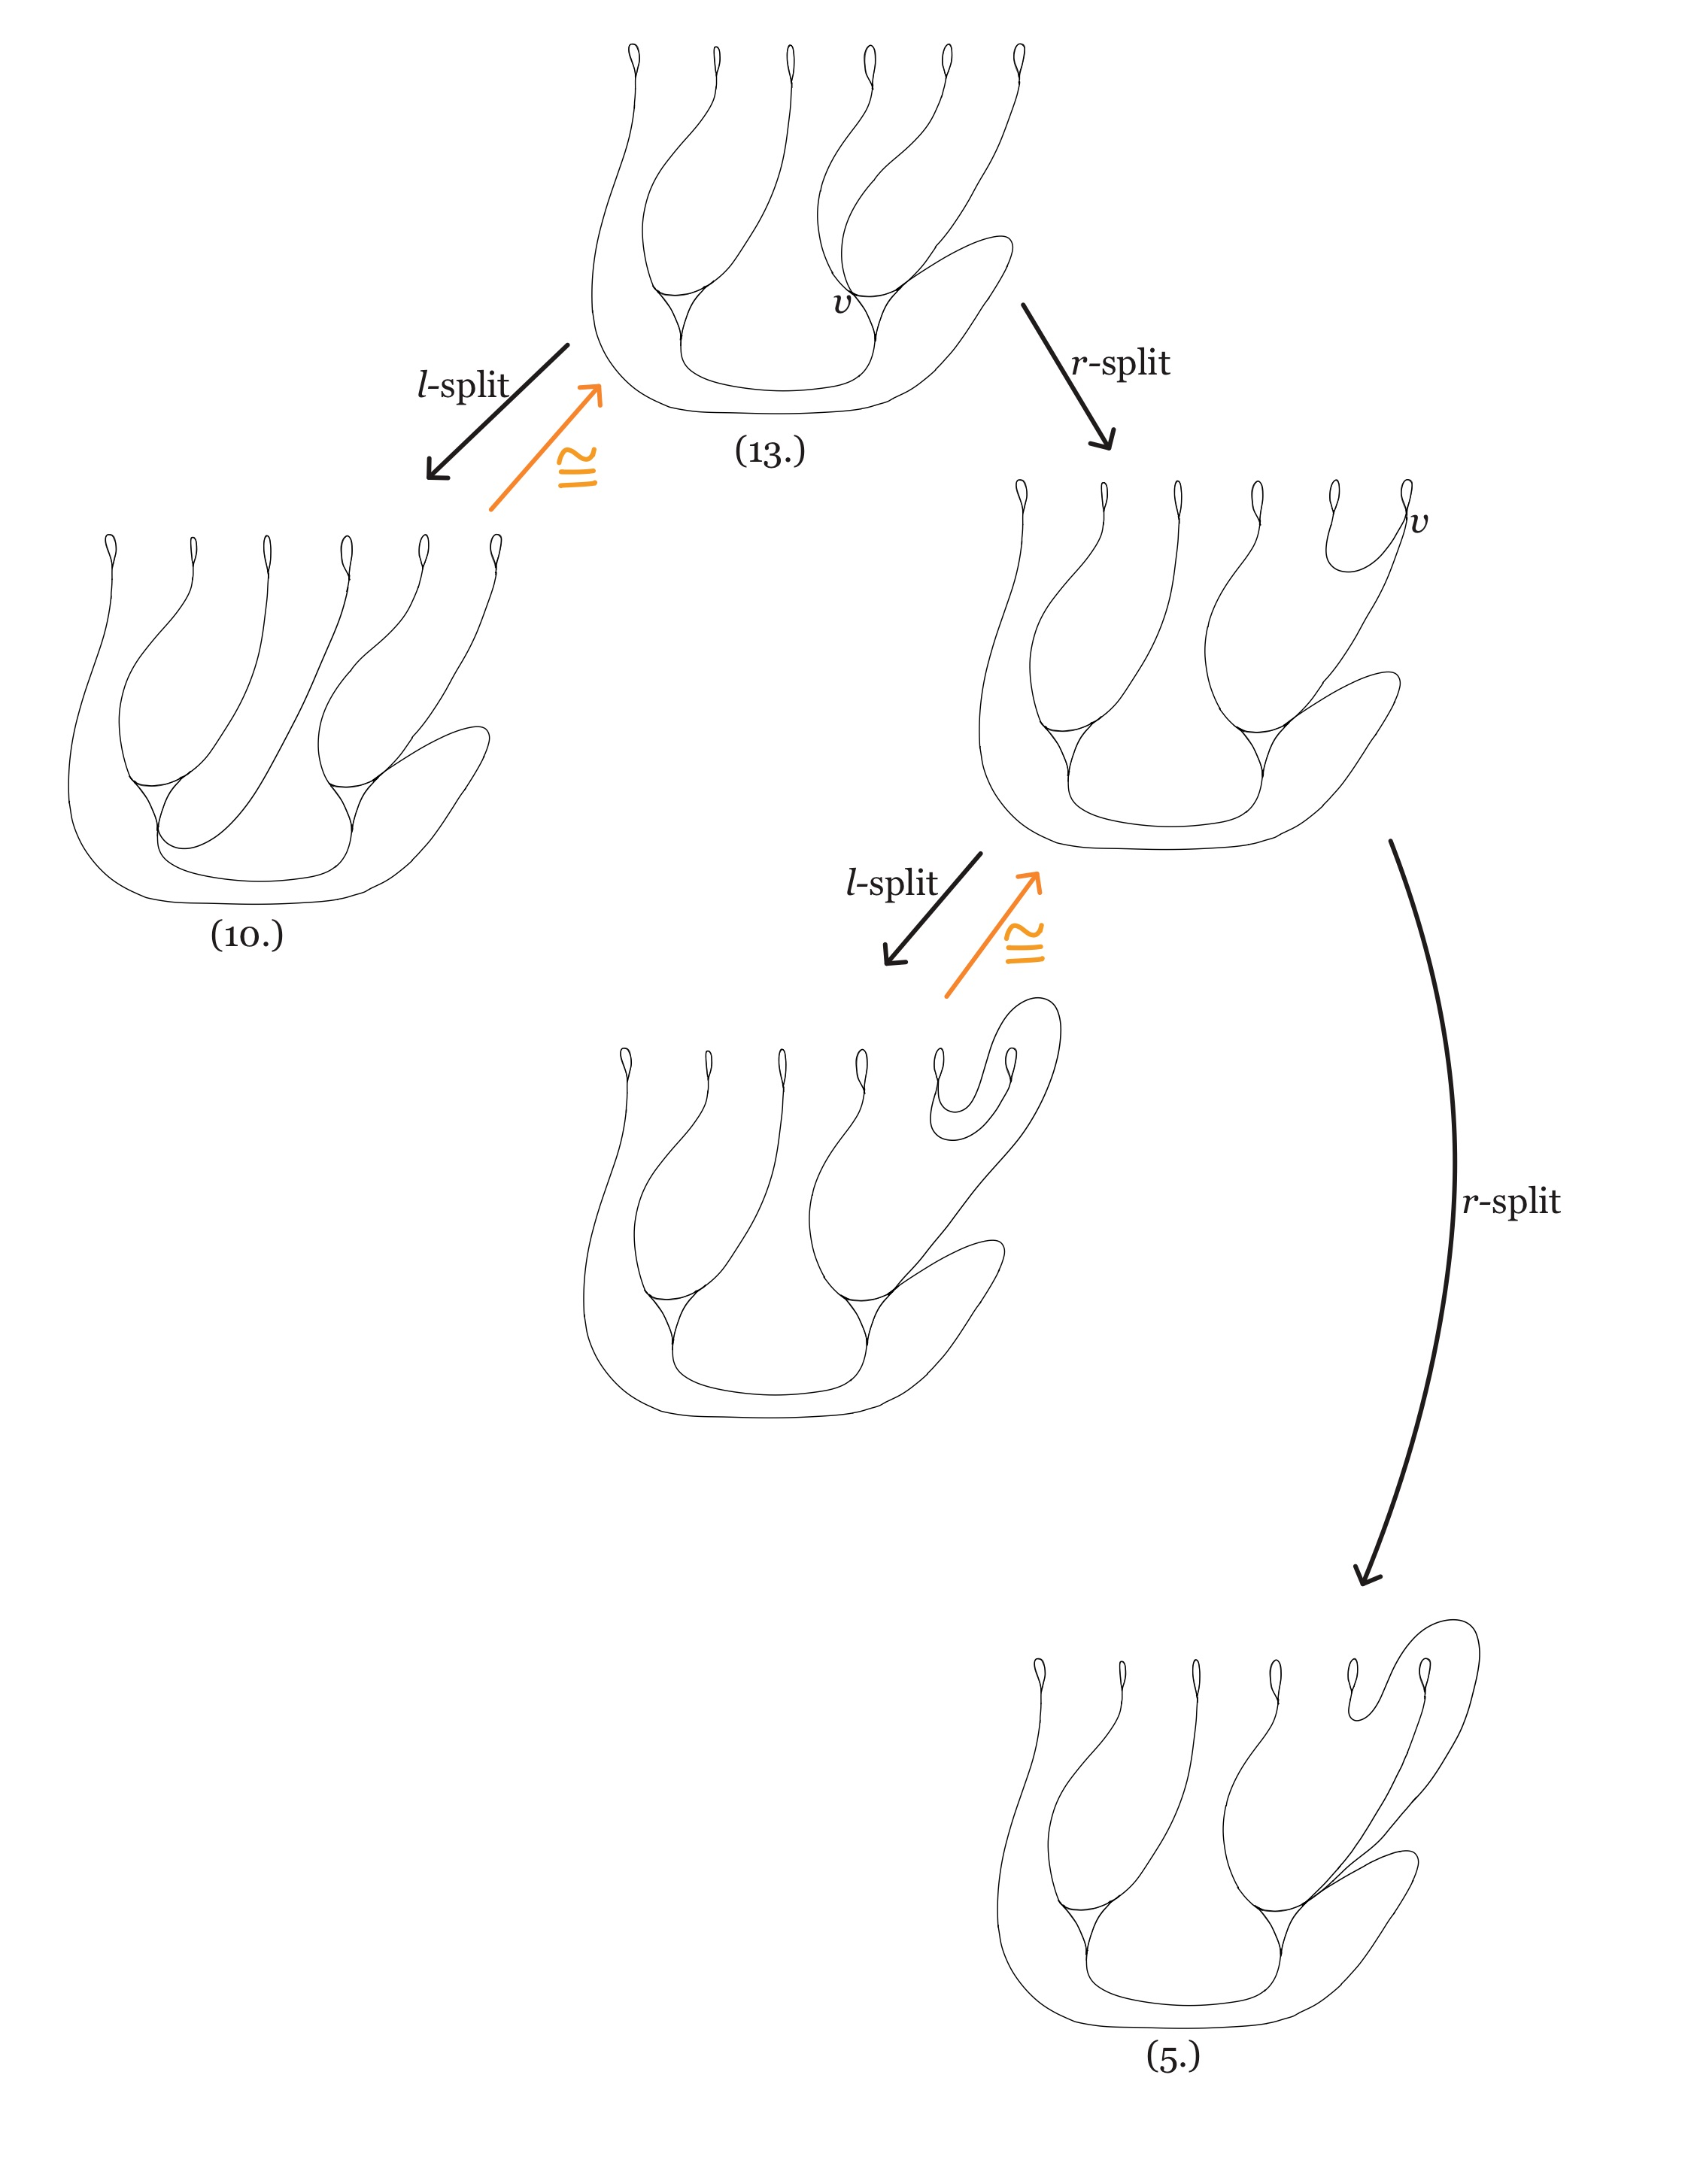
\includegraphics[width=\linewidth, height=0.45\textheight, keepaspectratio]{figures_splitting/13 Splitting-2.jpg}
    \caption{This splitting sequence shows train track (13.) eventually splits to the train tracks (8.), (6.), (10.), or (5.).}
    \label{fig:13_splitting}
\end{figure*}

\begin{figure*}[p] % [p] forces this to be on its own page, which is often necessary for large figures
    \centering
    % Restrict height to 45% of the text block per image, maintaining aspect ratio
    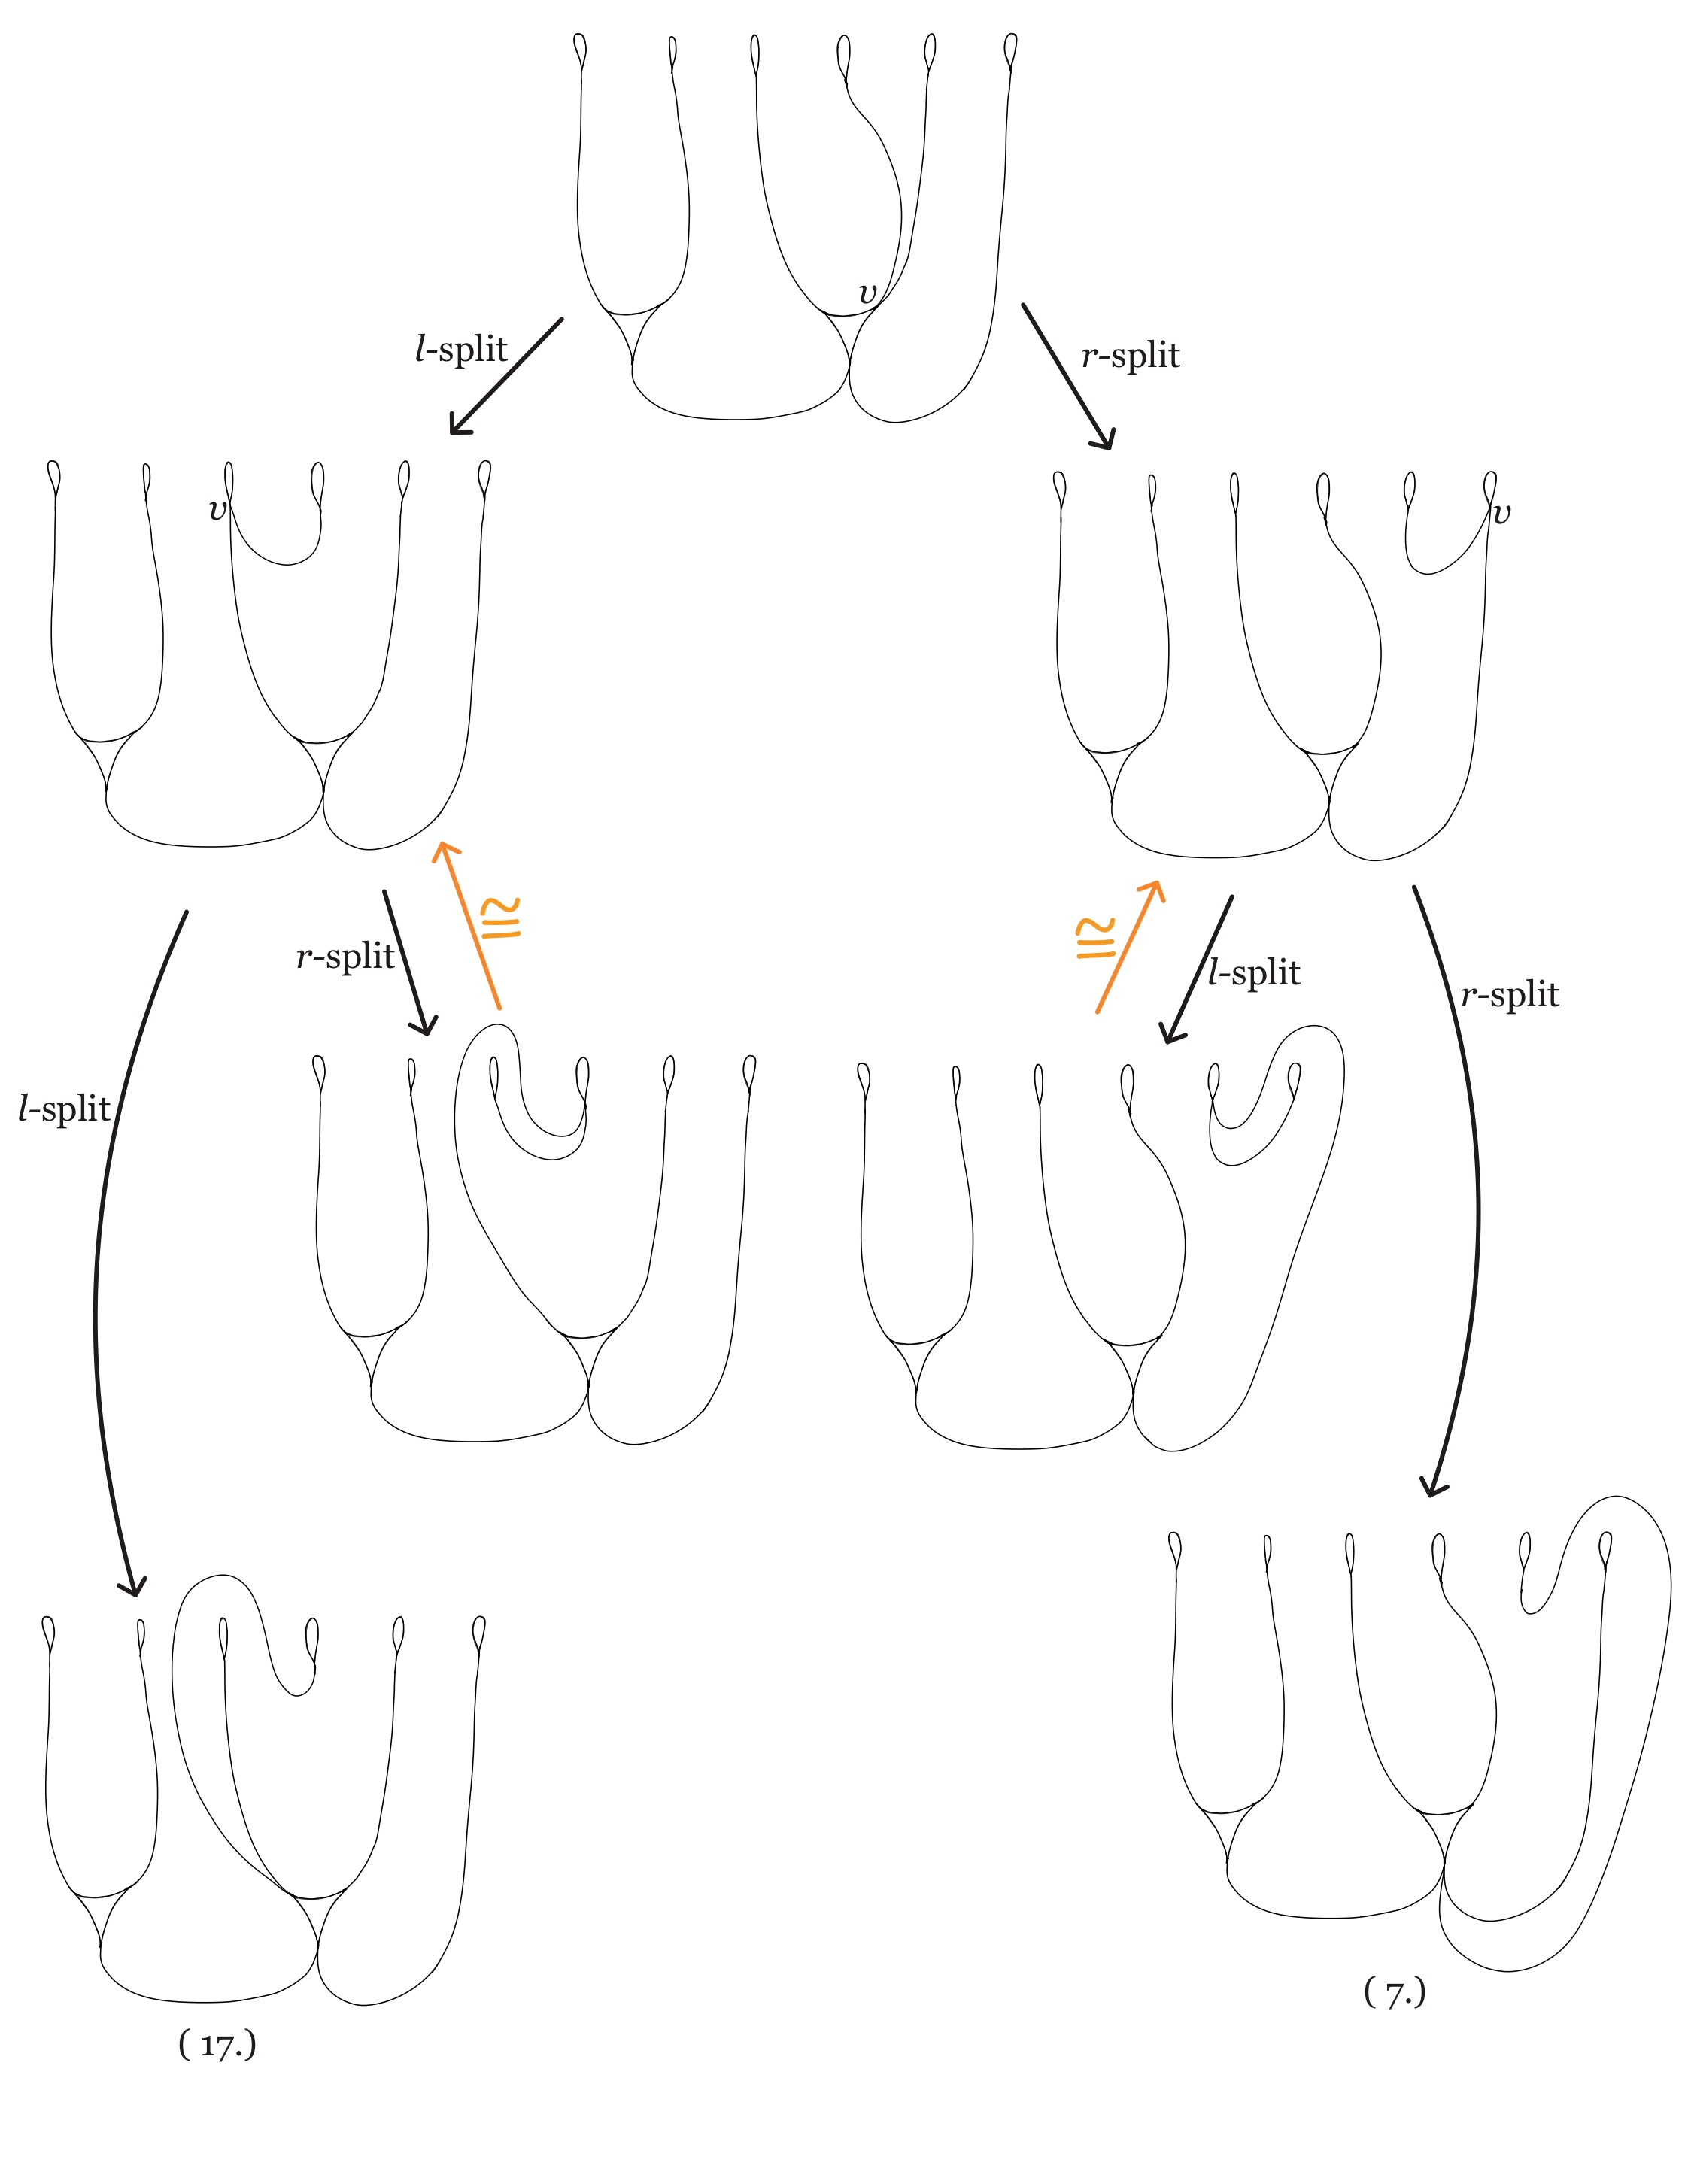
\includegraphics[width=\linewidth, height=0.45\textheight, keepaspectratio]{figures_splitting/12 Splitting-1.jpg}\\[0pt]
    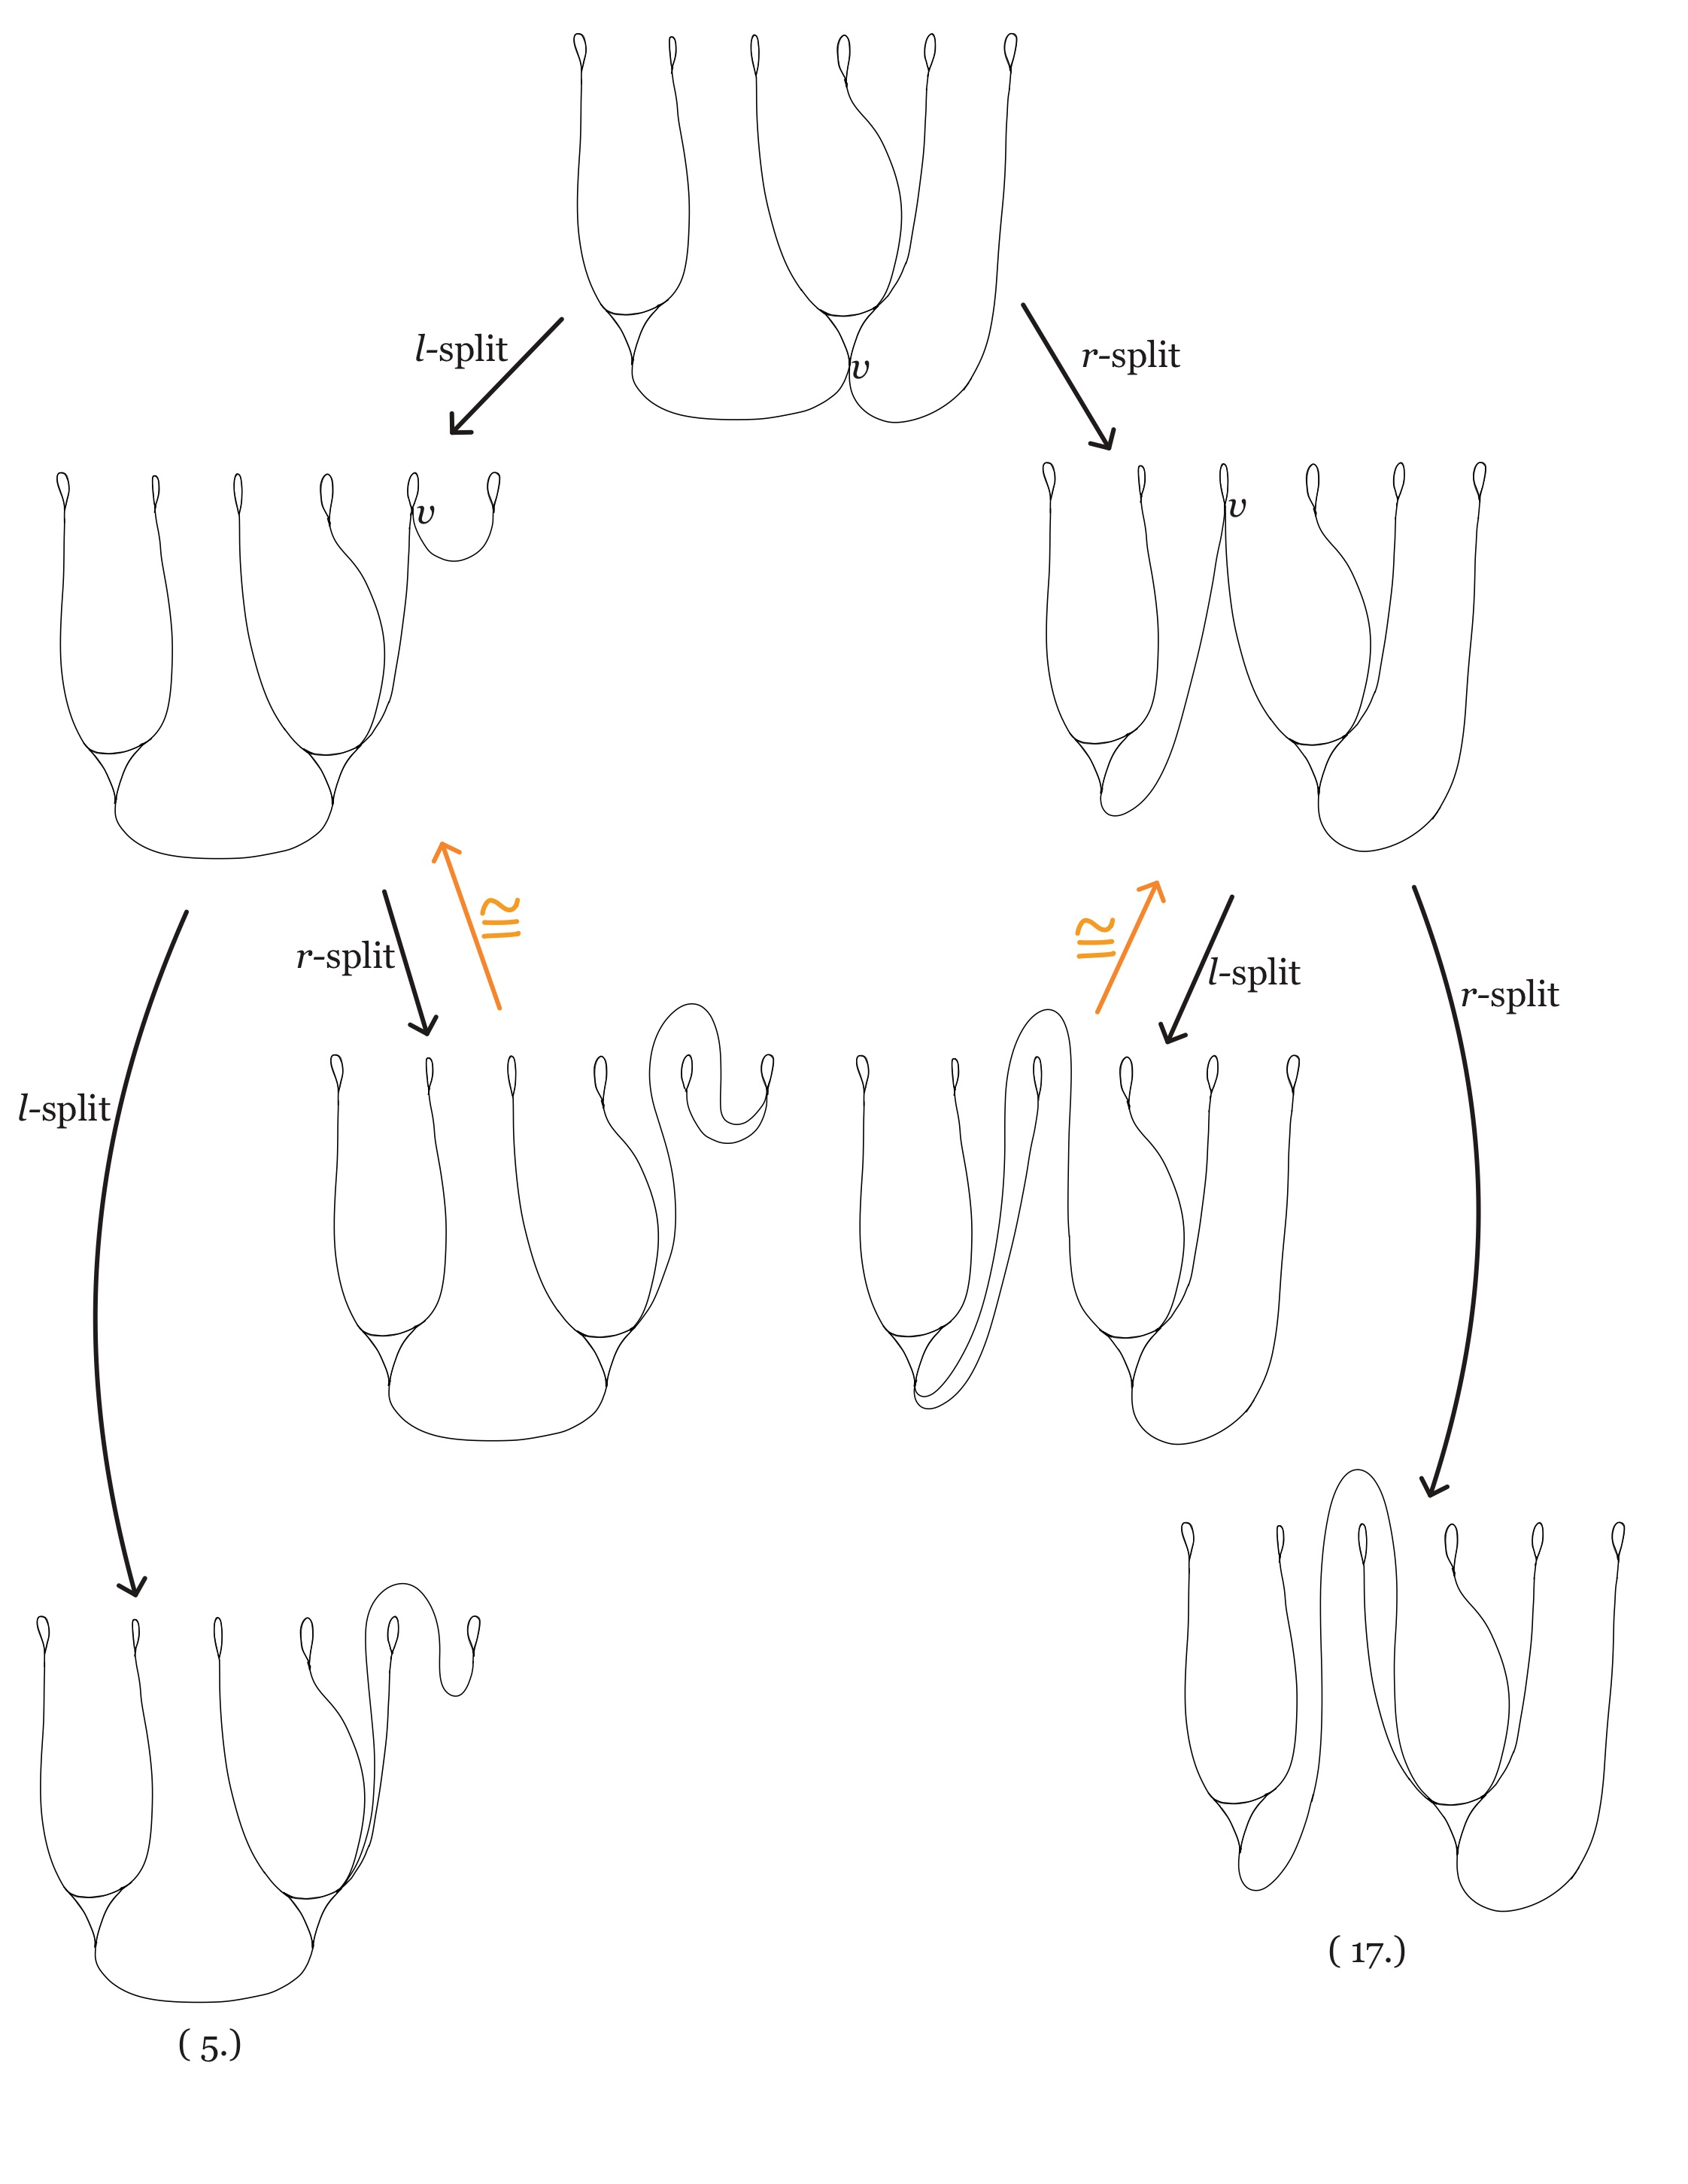
\includegraphics[width=\linewidth, height=0.45\textheight, keepaspectratio]{figures_splitting/12 Splitting-2.jpg}
    \caption{This splitting sequence shows train track (12.) eventually splits to the train tracks (17.), (7.), or (5.).}
    \label{fig:12_splitting}
\end{figure*}

\begin{figure*}[p] % [p] forces this to be on its own page, which is often necessary for large figures
    \centering
    % Restrict height to 45% of the text block per image, maintaining aspect ratio
    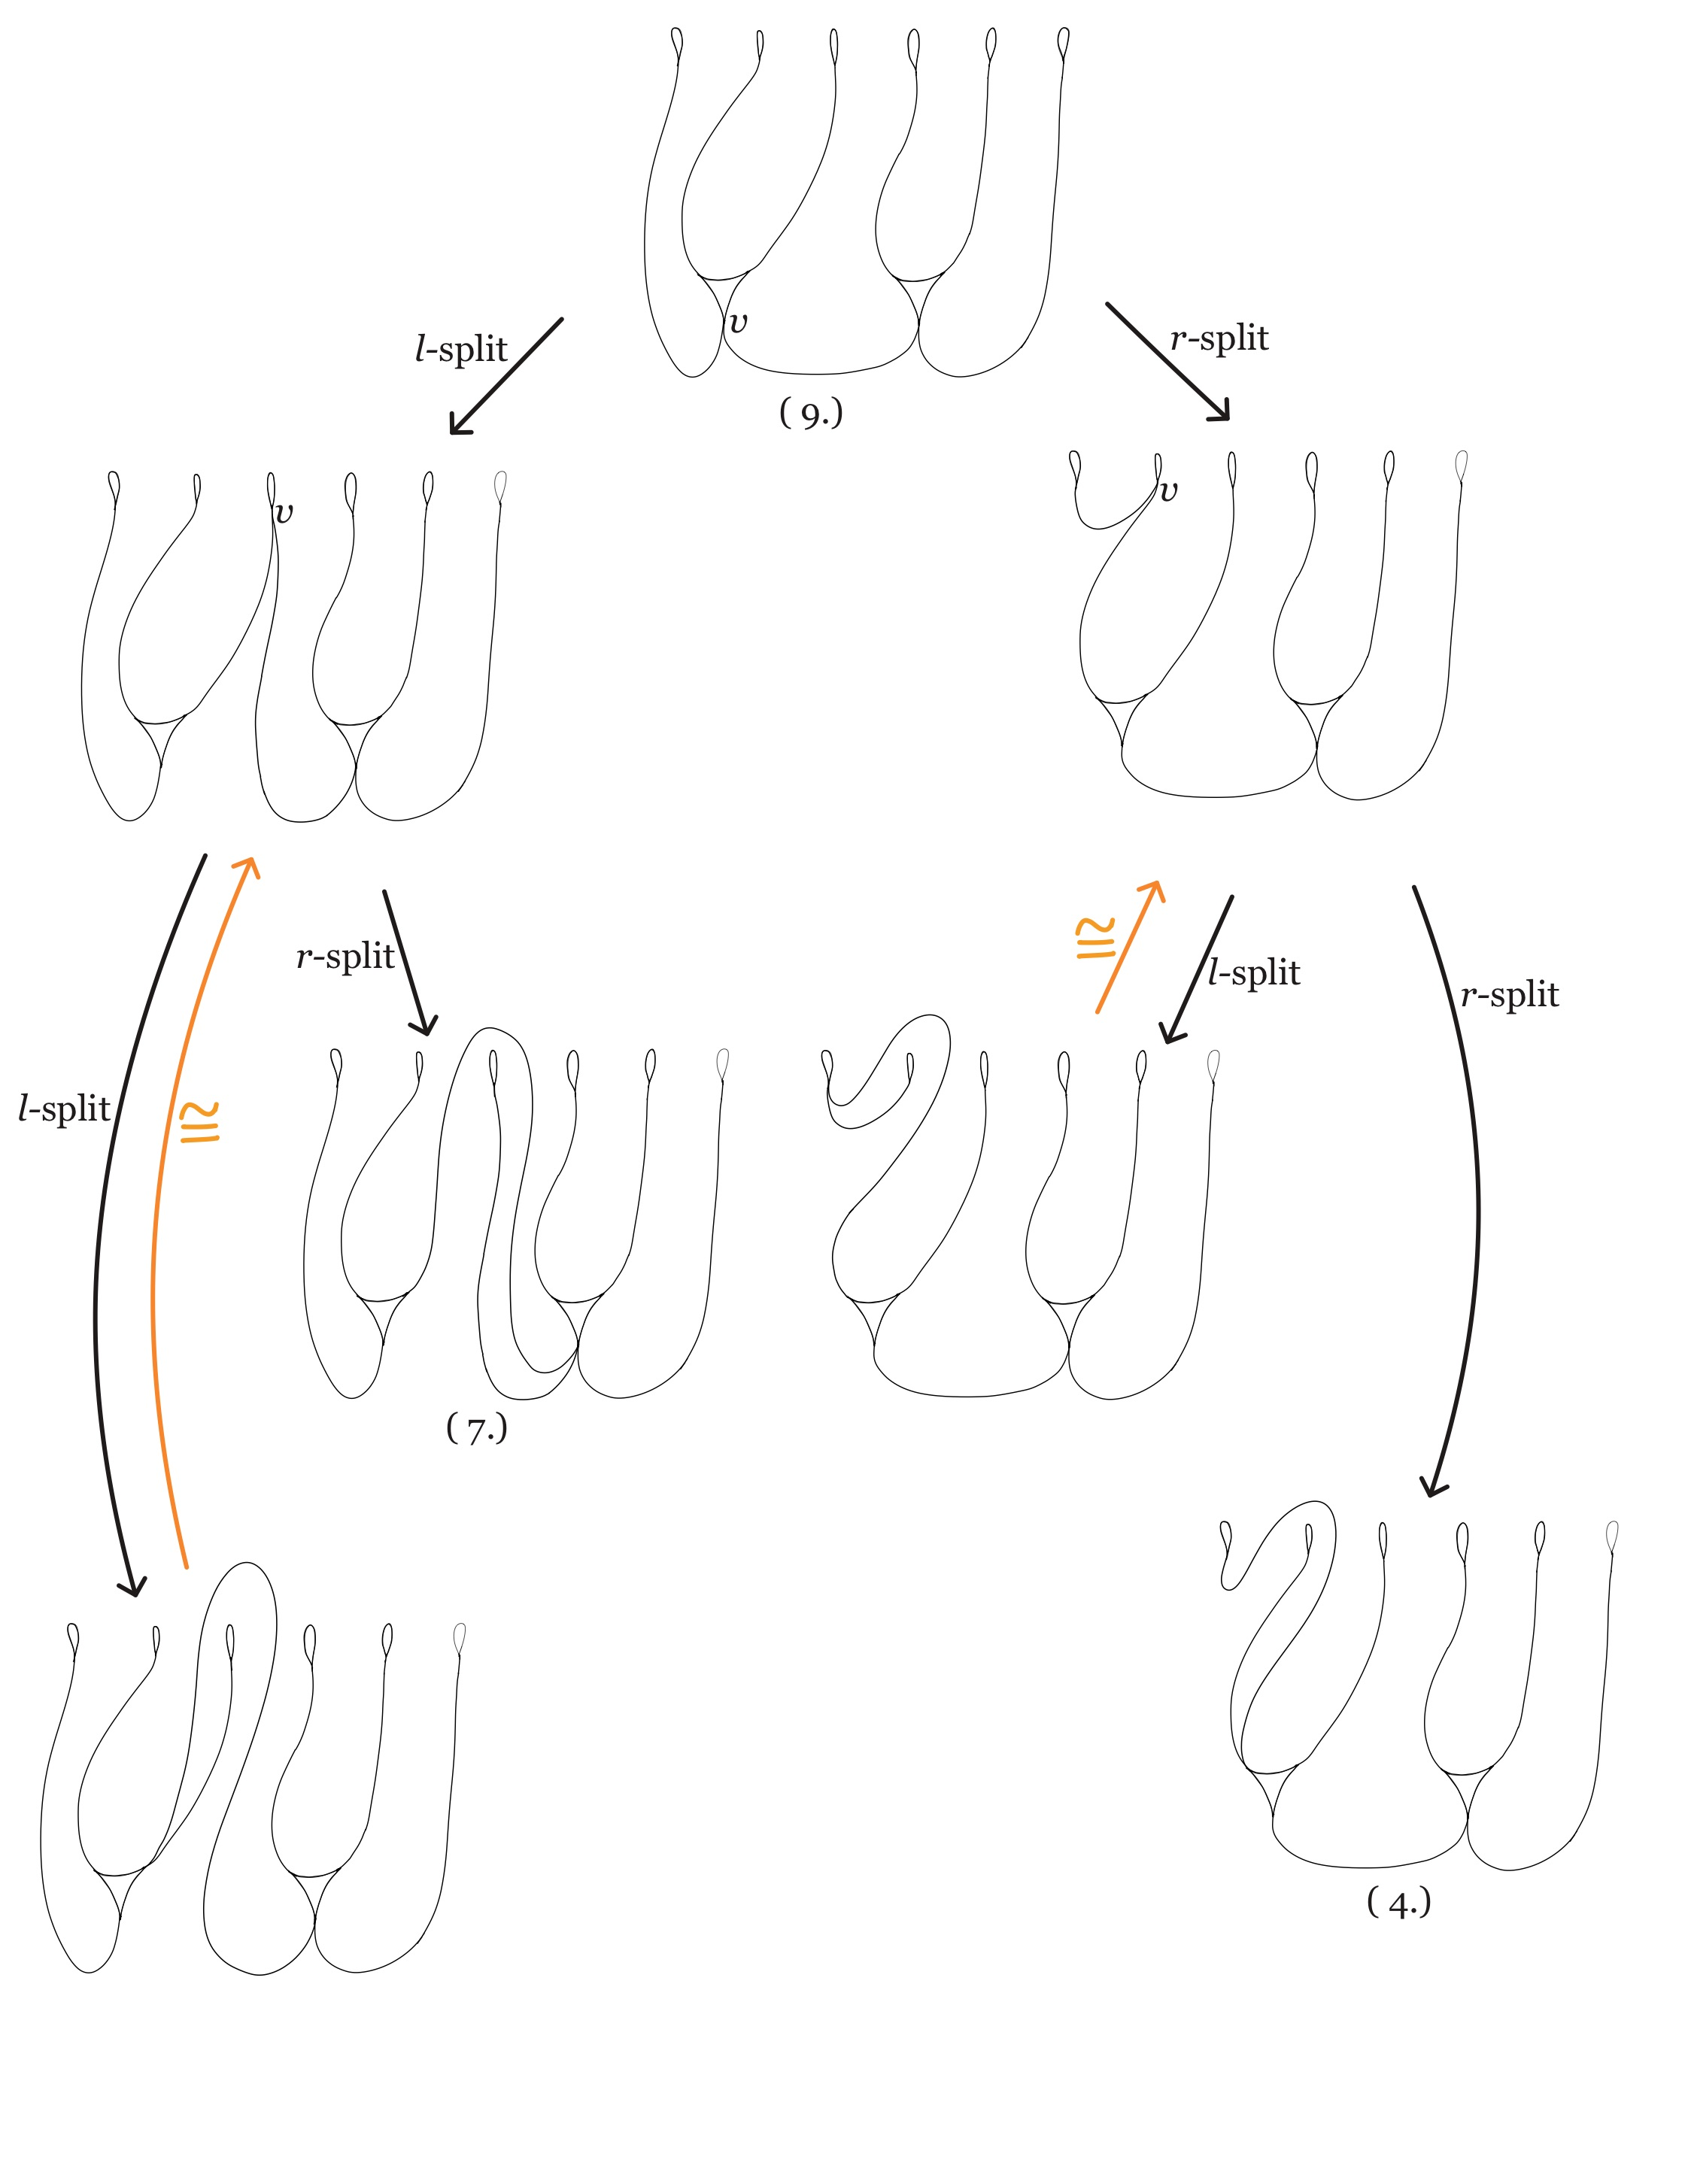
\includegraphics[width=\linewidth, height=0.45\textheight, keepaspectratio]{figures_splitting/9 Splitting-1.jpg}\\[0pt]
    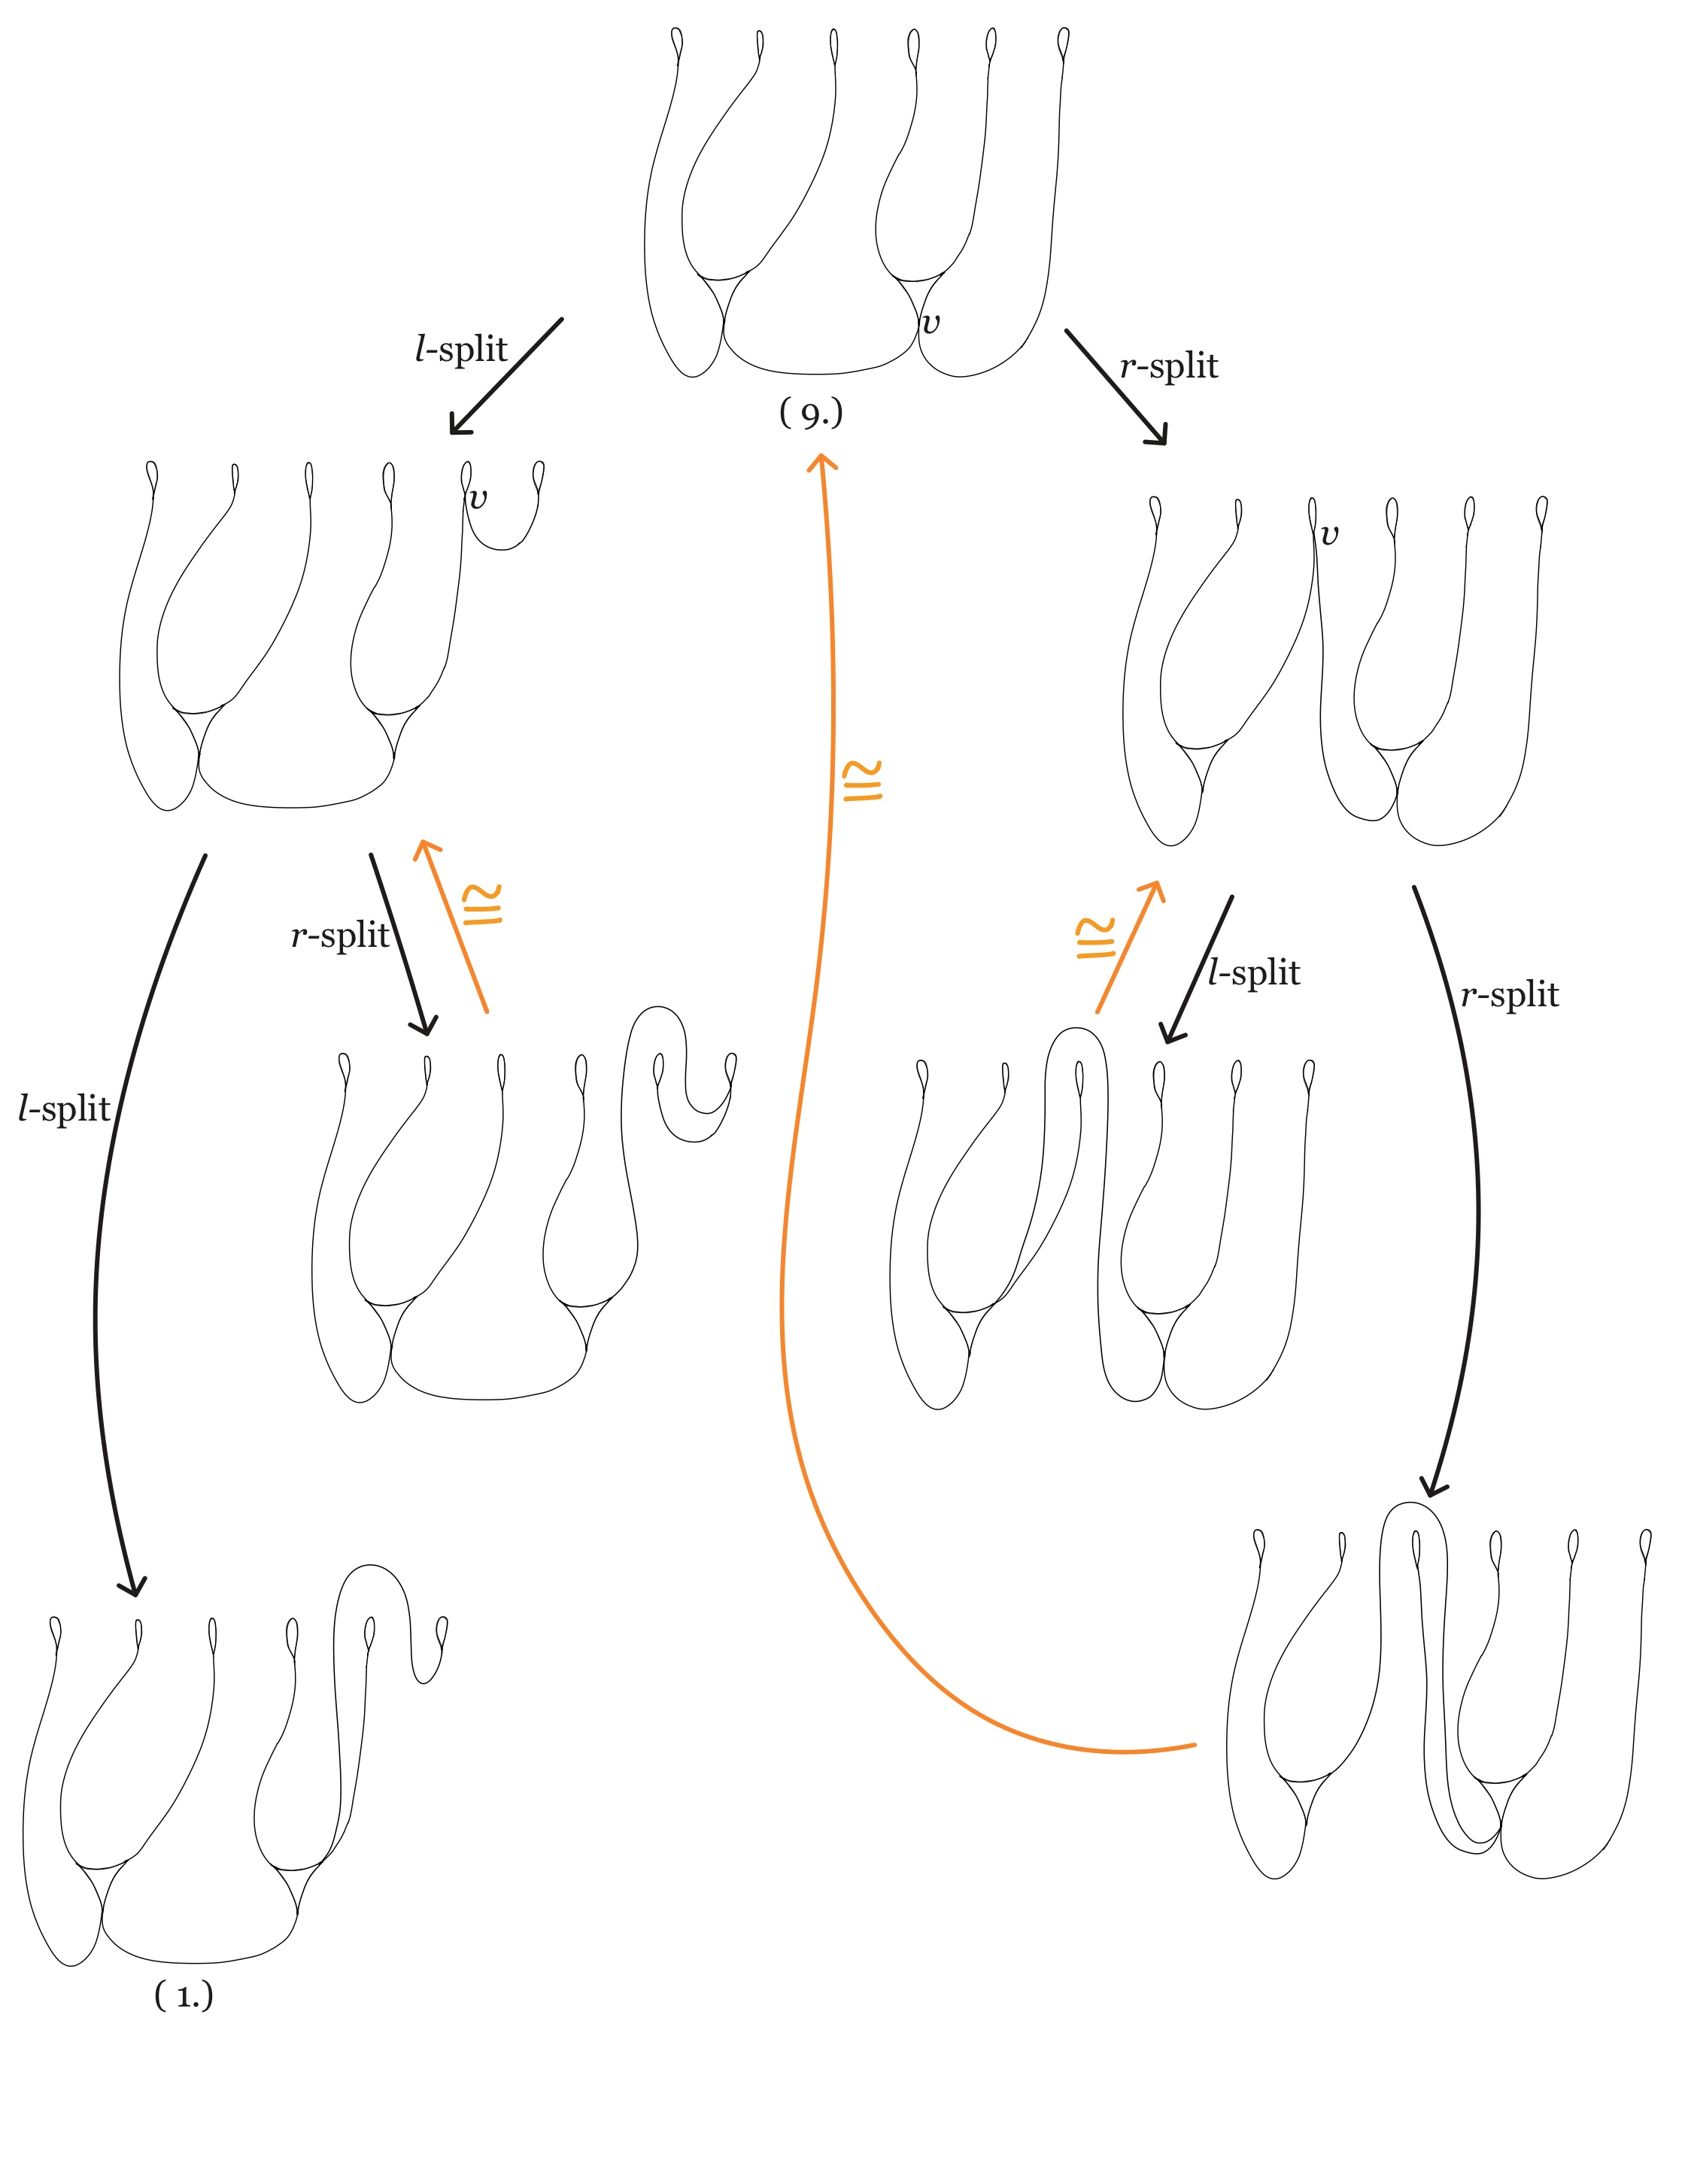
\includegraphics[width=\linewidth, height=0.45\textheight, keepaspectratio]{figures_splitting/9 Splitting-2.jpg}
    \caption{This splitting sequence shows train track (9.) eventually splits to the train tracks (7.), (4.), or (1.).}
    \label{fig:9_splitting}
\end{figure*}

\begin{figure*}[p] % [p] forces this to be on its own page, which is often necessary for large figures
    \centering
    % Restrict height to 45% of the text block per image, maintaining aspect ratio
    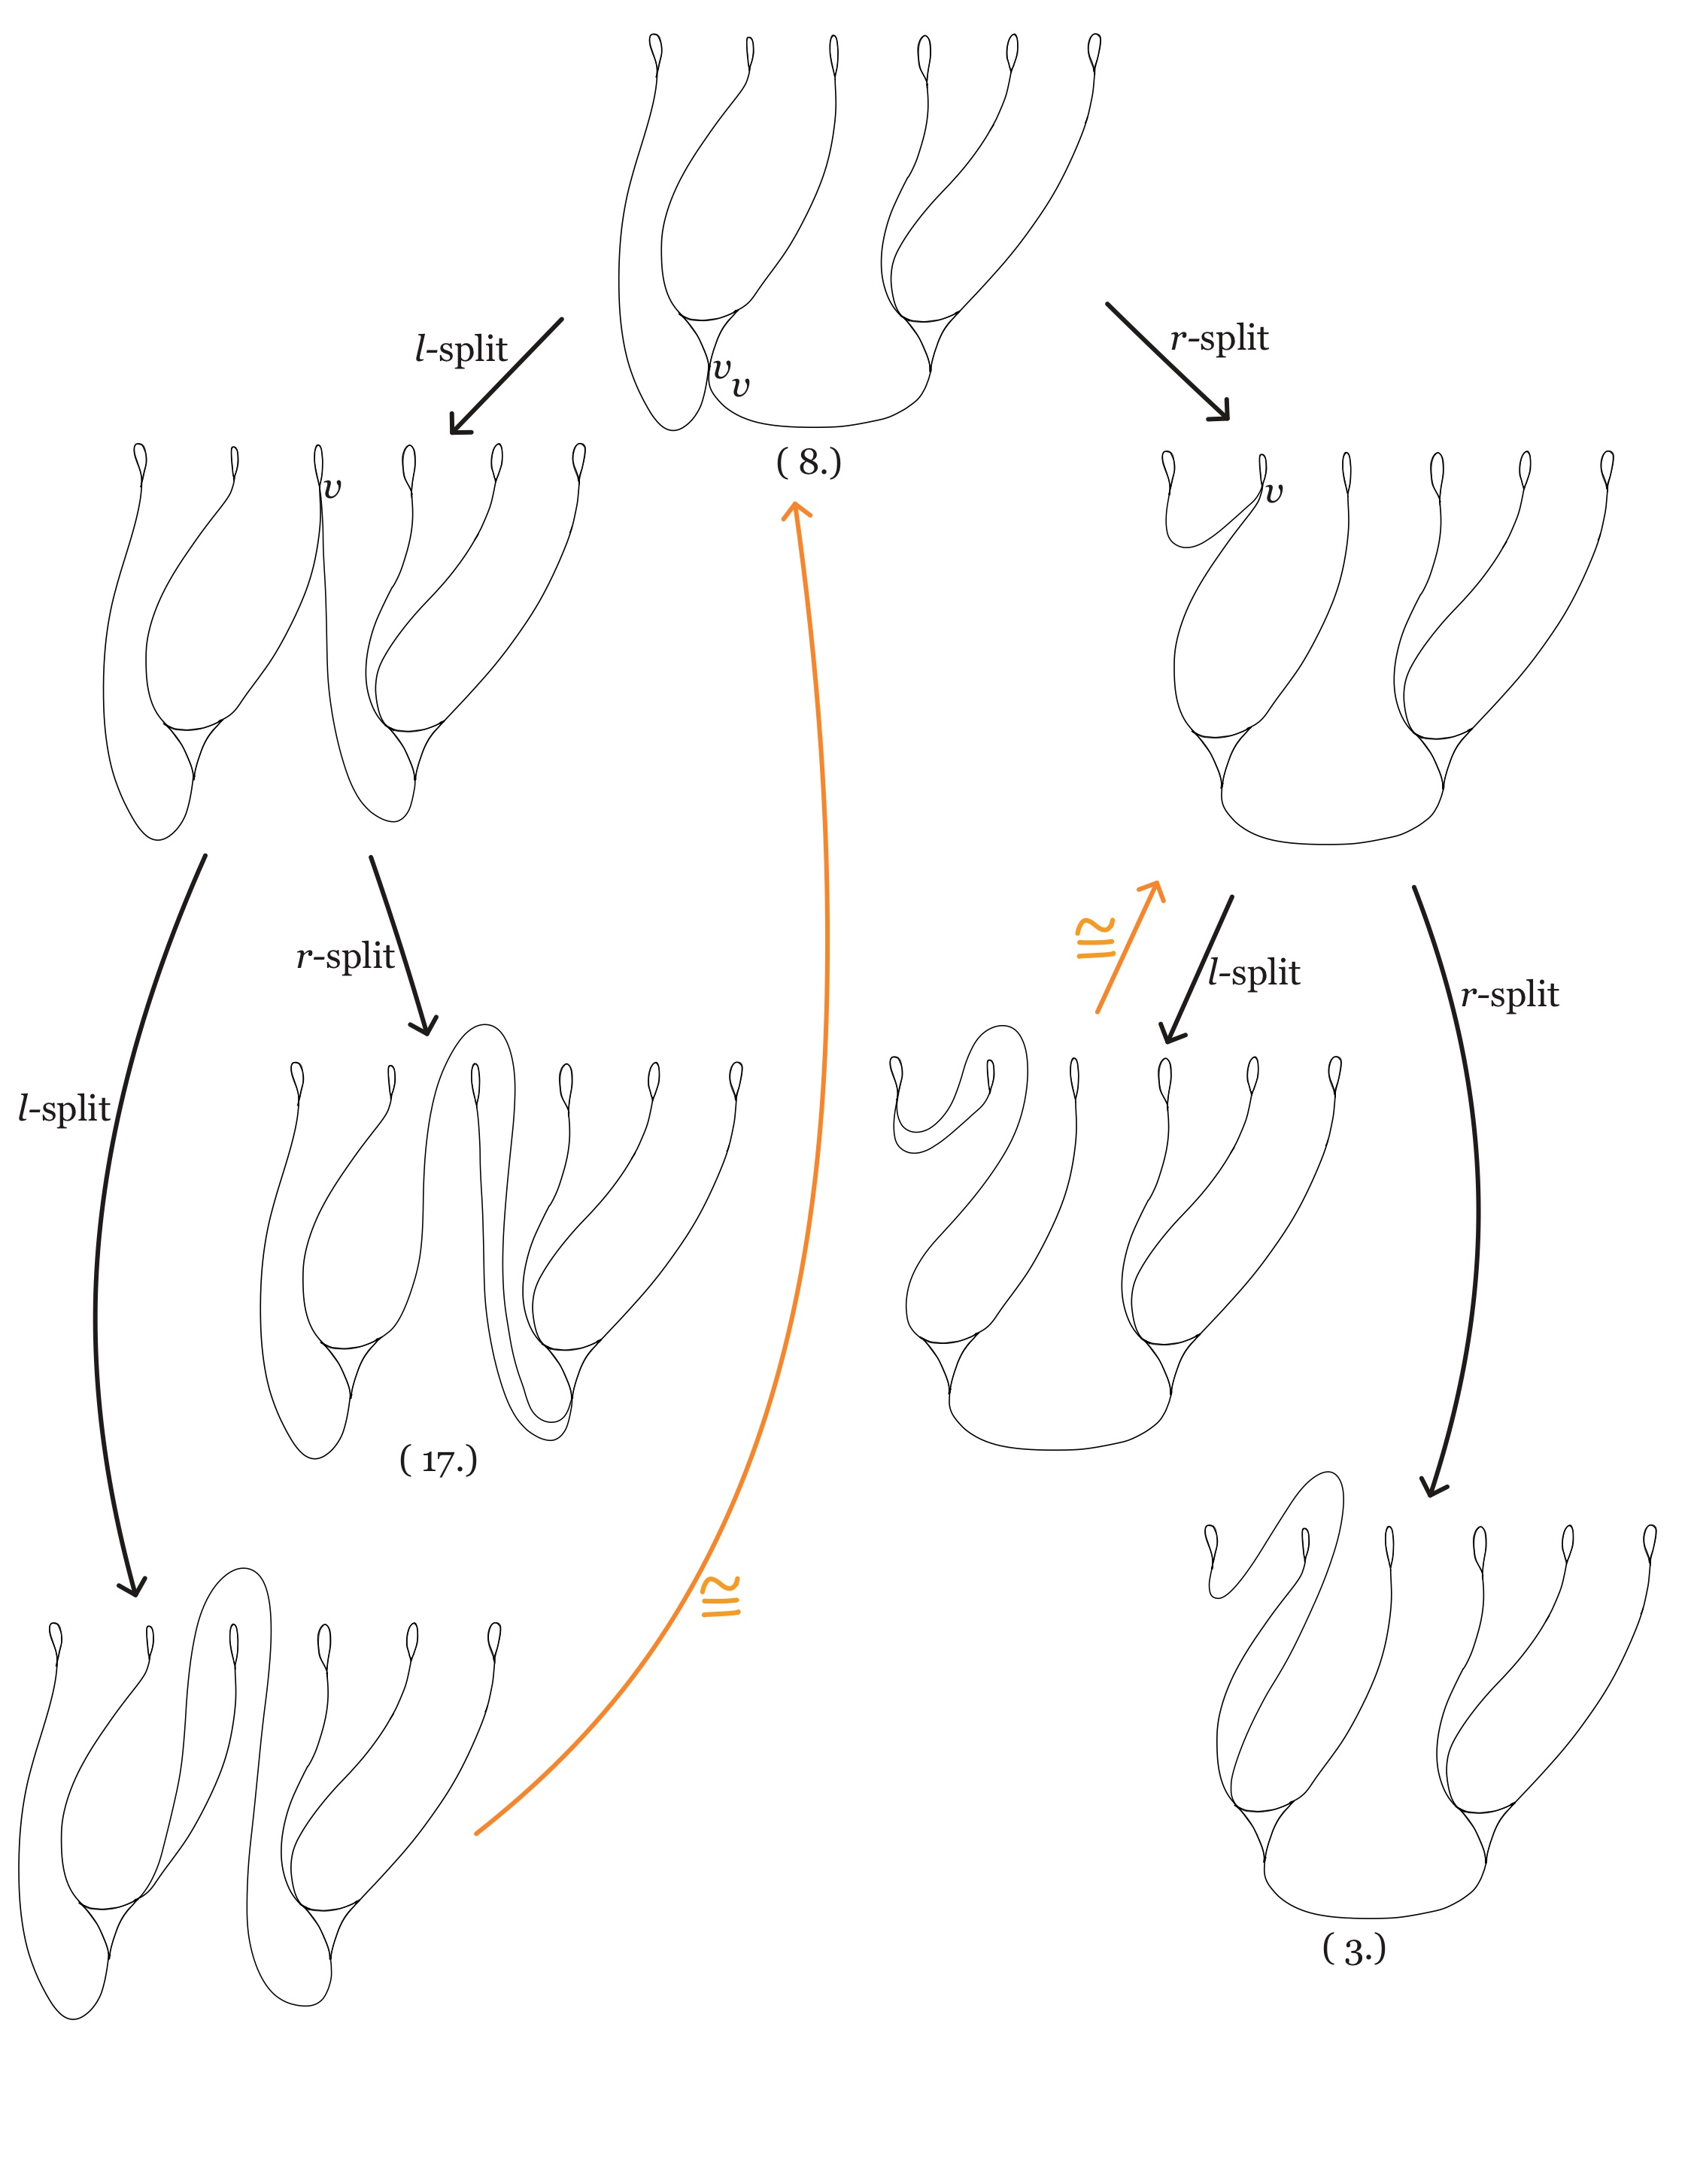
\includegraphics[width=\linewidth, height=0.45\textheight, keepaspectratio]{figures_splitting/8 Splitting-1.jpg}\\[0pt]
    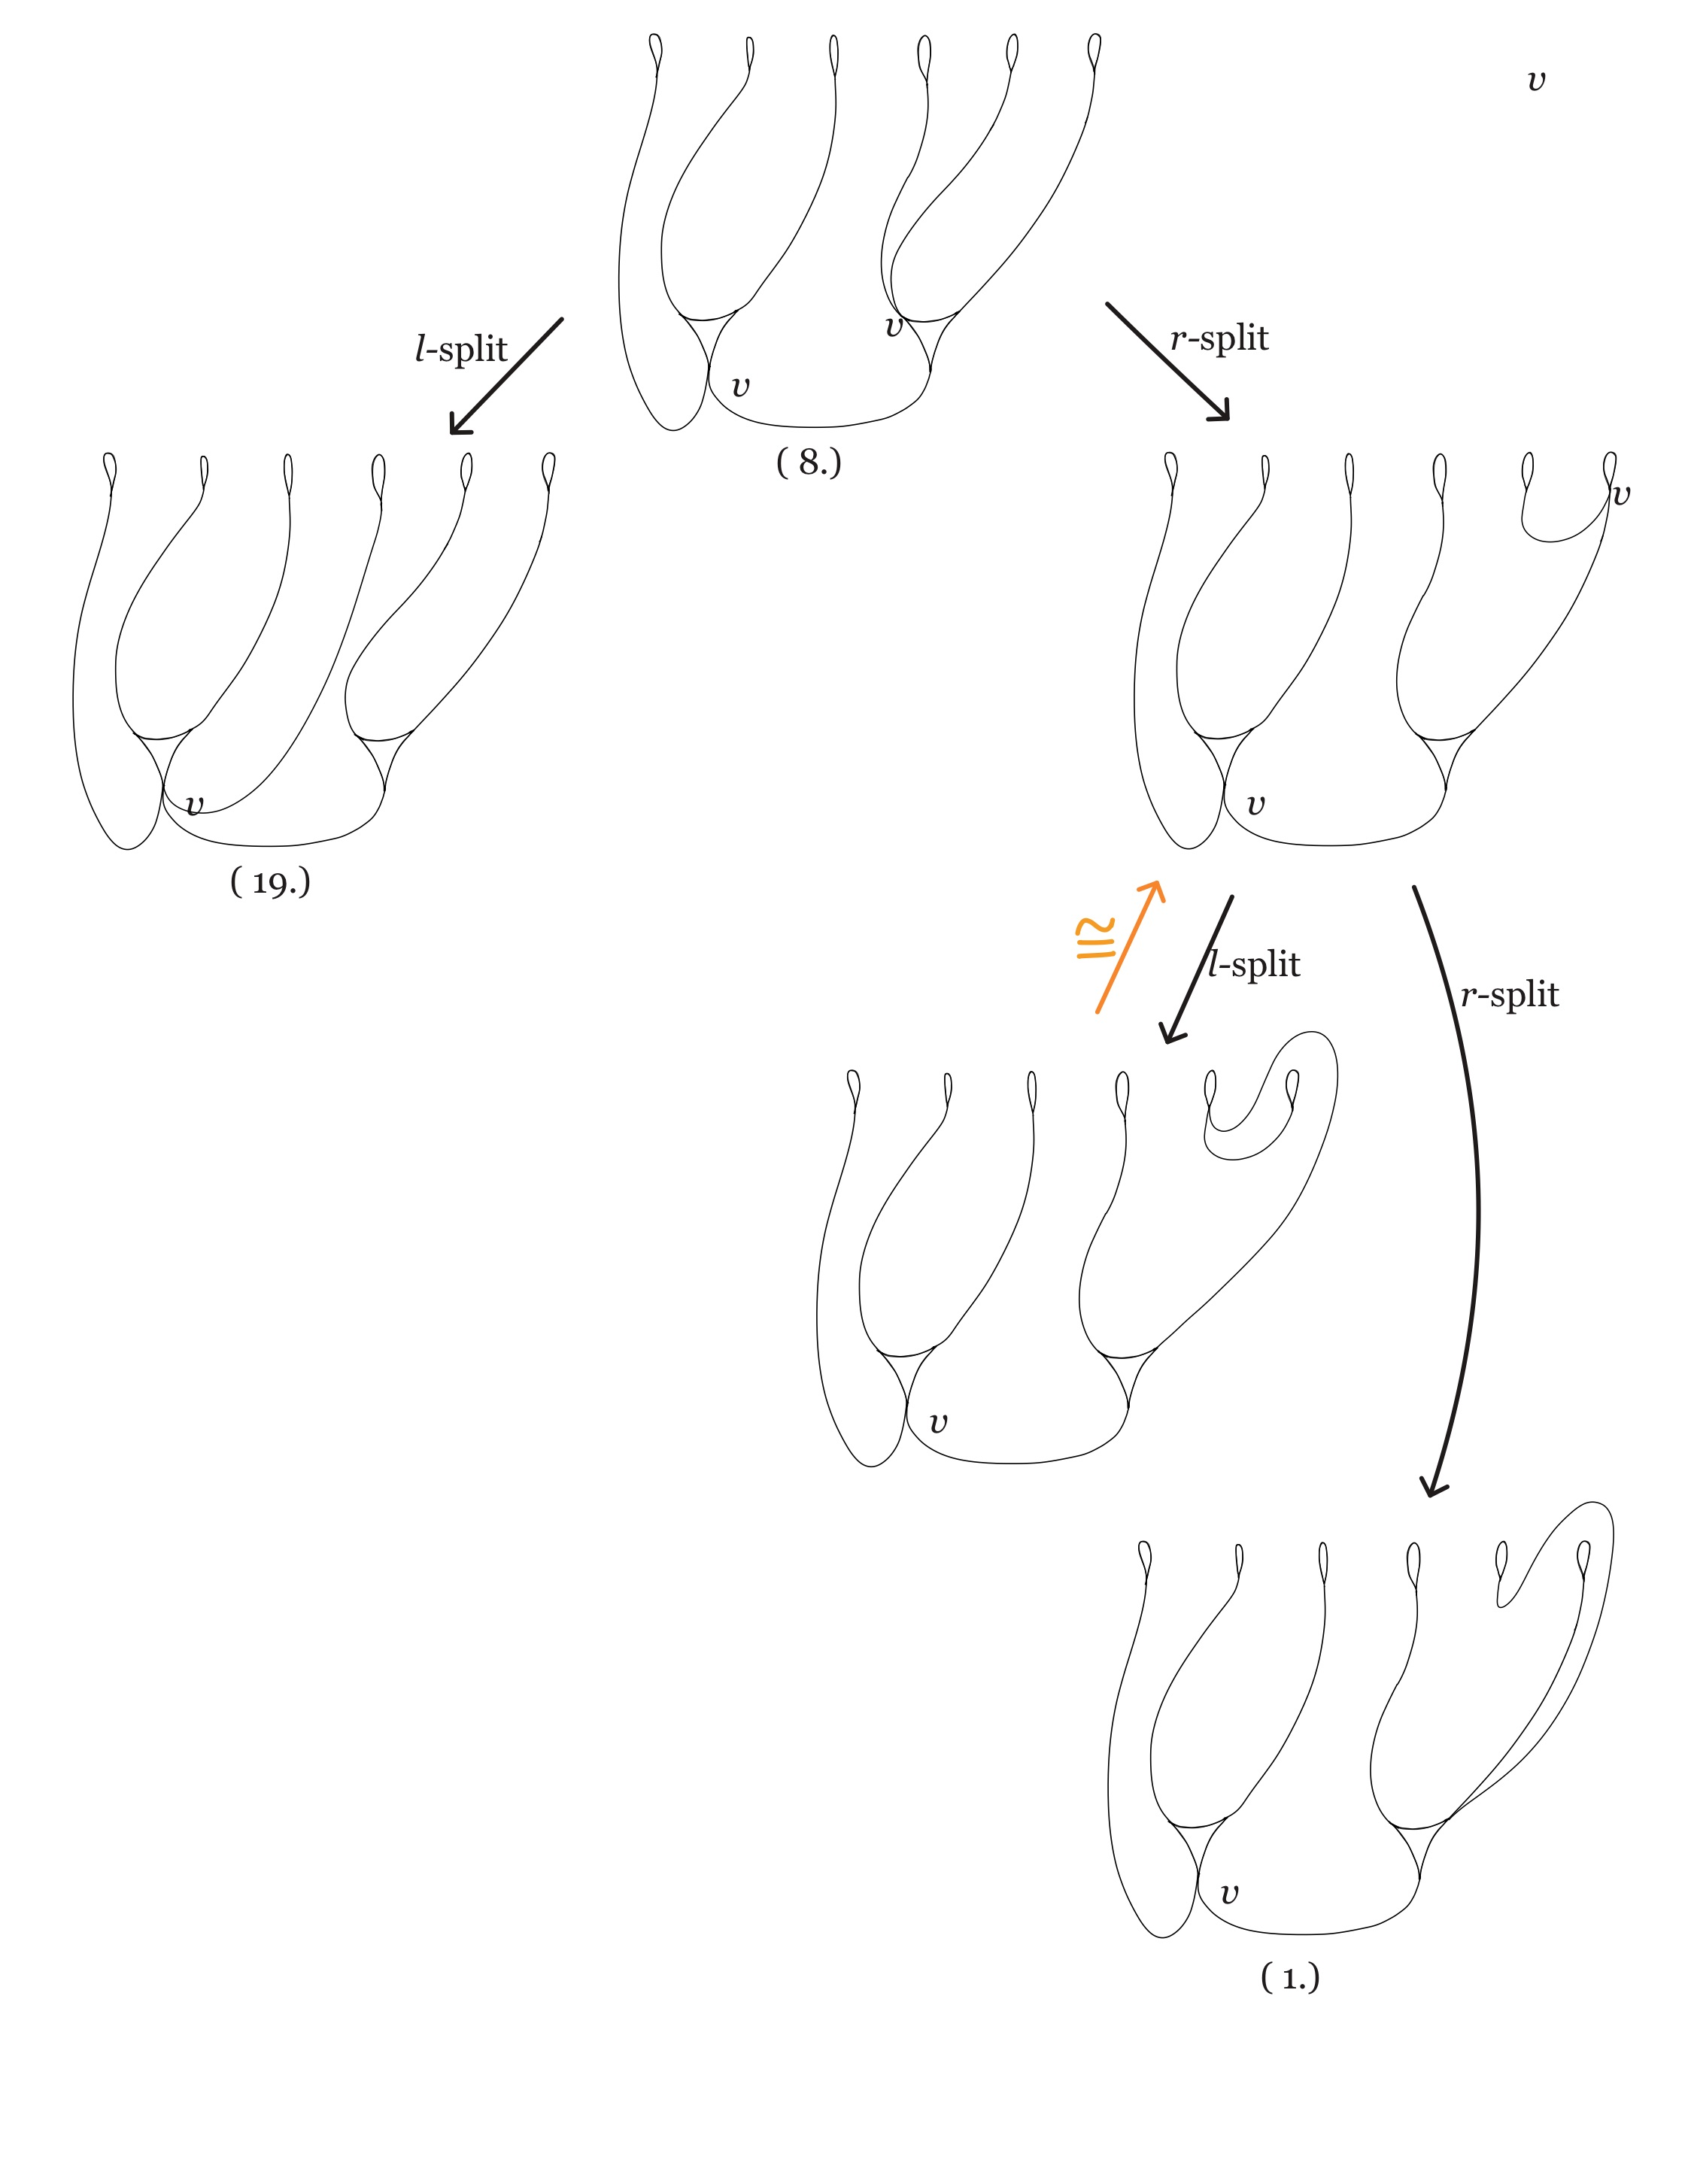
\includegraphics[width=\linewidth, height=0.45\textheight, keepaspectratio]{figures_splitting/8 Splitting-2.jpg}
    \caption{This splitting sequence shows train track (8.) eventually splits to the train tracks (17.), (3.), (19.), or (1.).}
    \label{fig:8_splitting}
\end{figure*}

\begin{figure*}[p] % [p] forces this to be on its own page, which is often necessary for large figures
    \centering
    % Restrict height to 45% of the text block per image, maintaining aspect ratio
    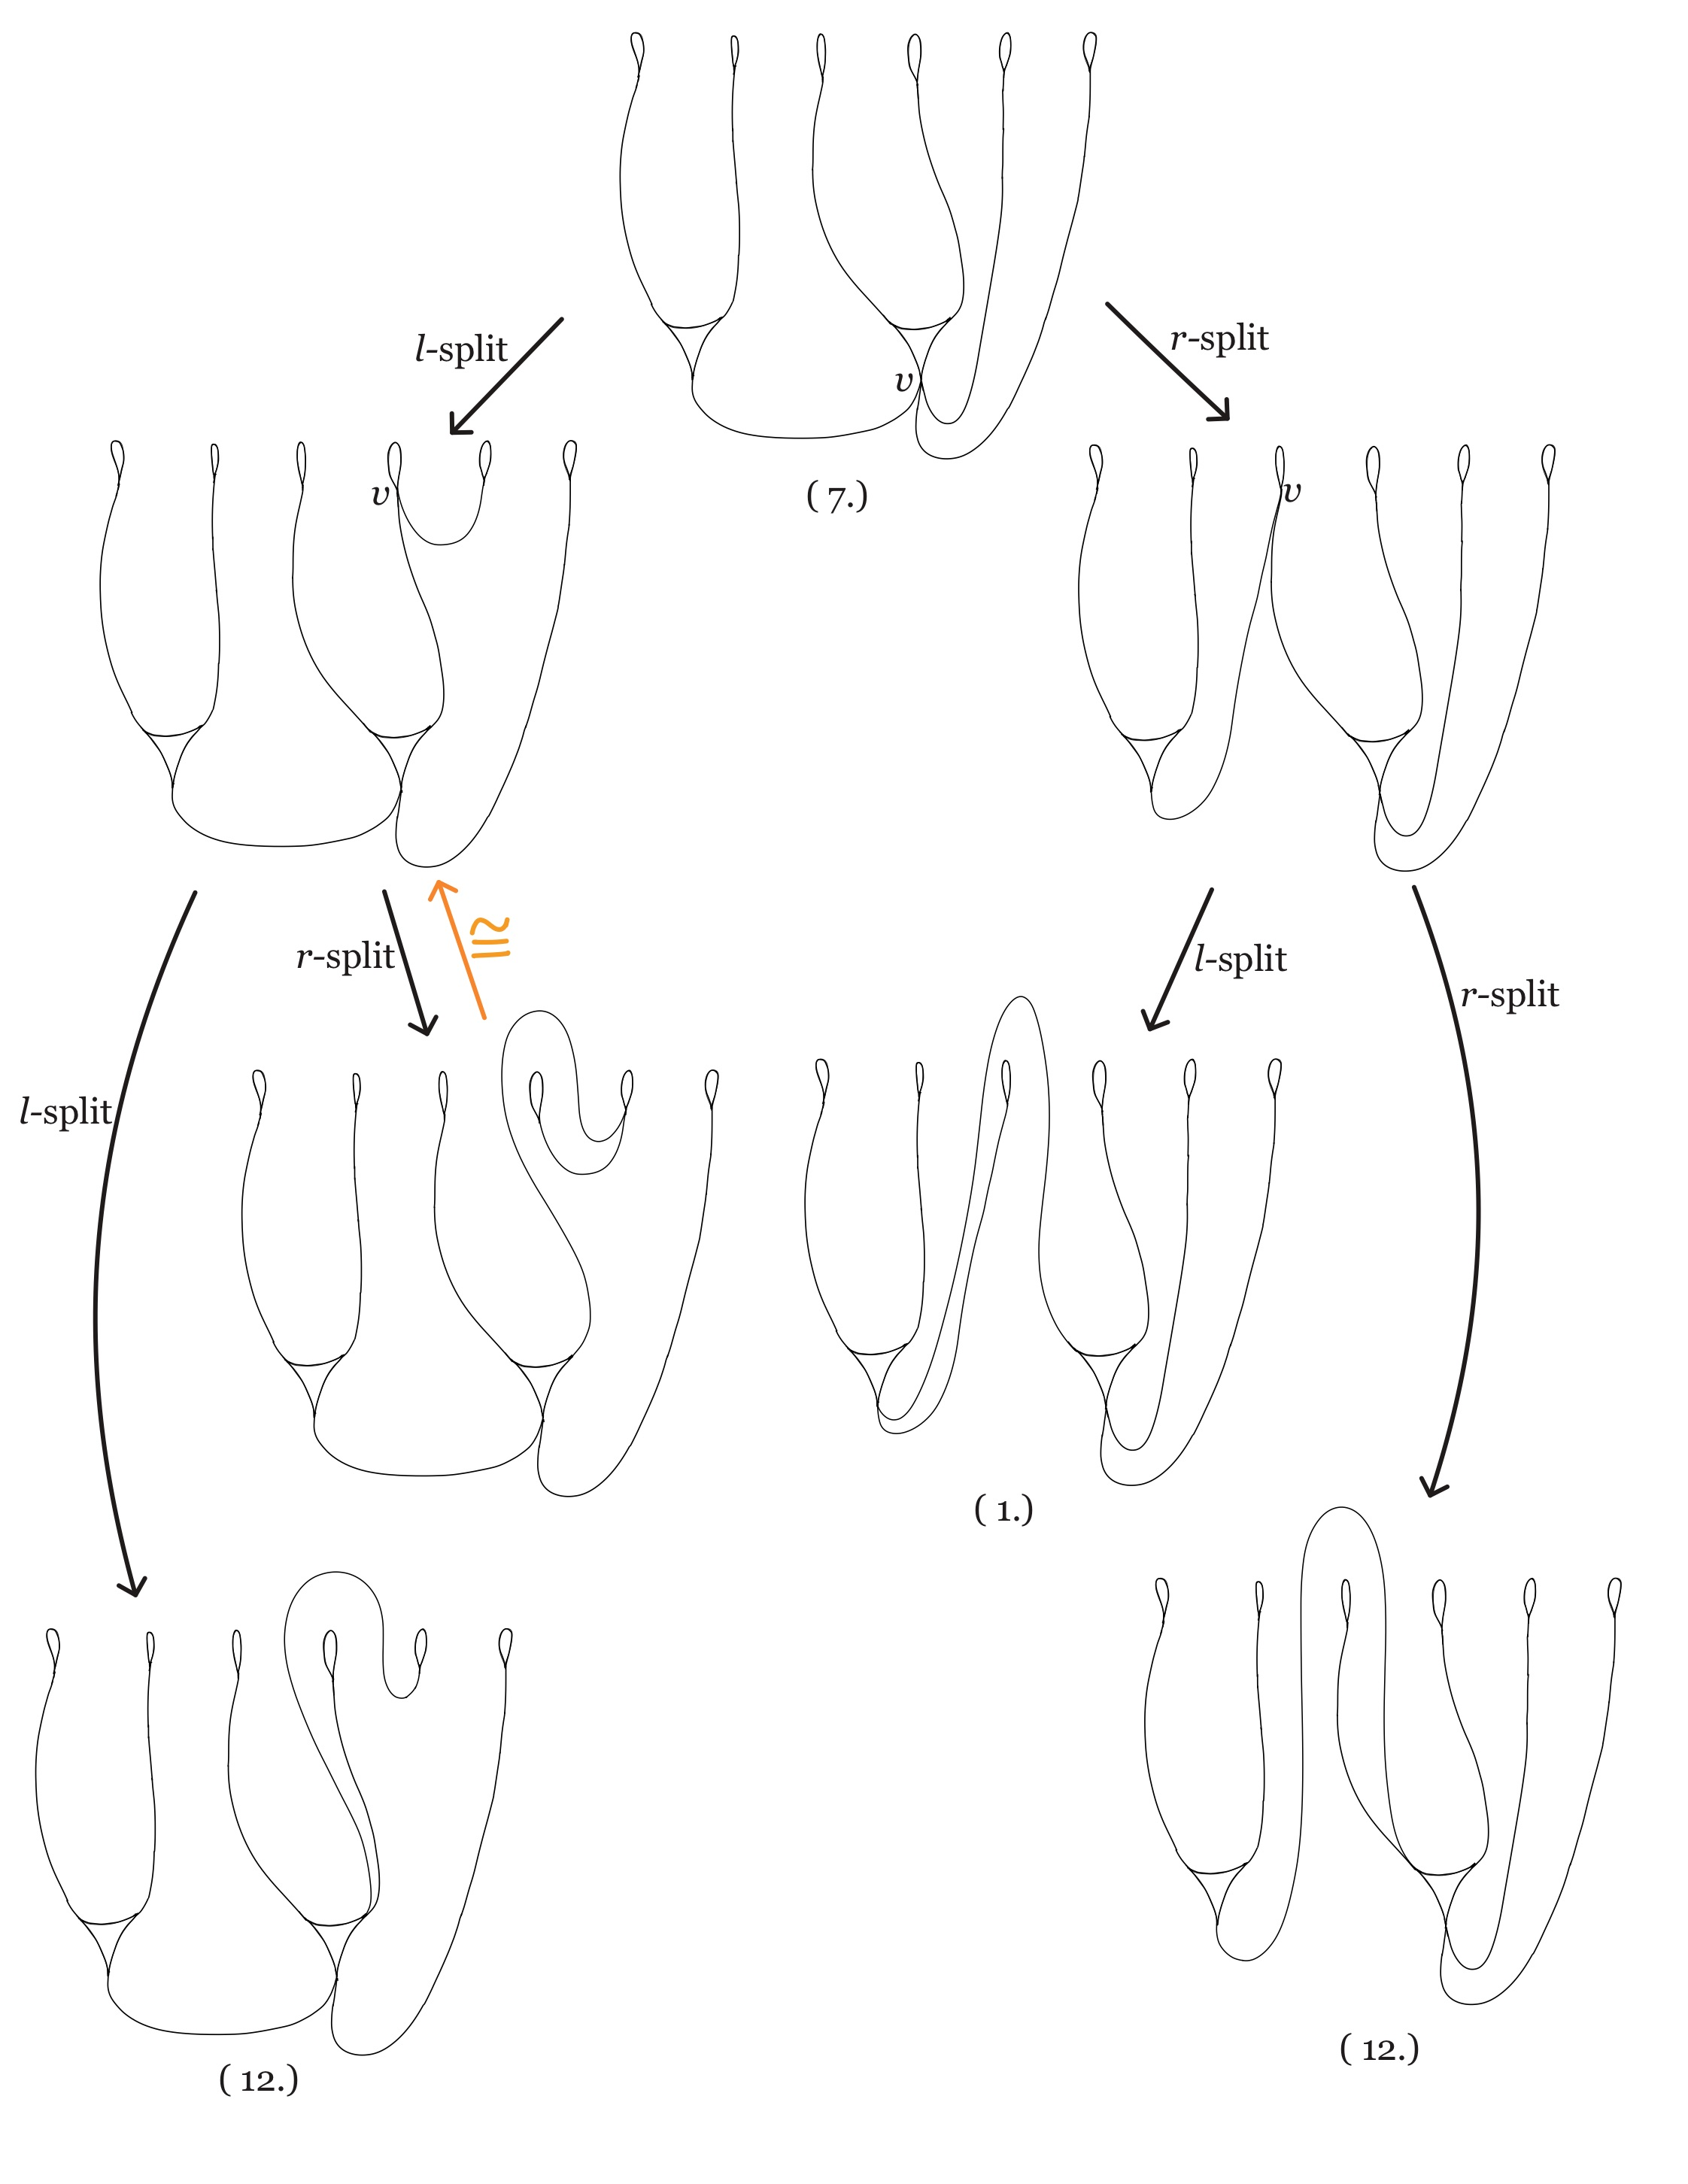
\includegraphics[width=\linewidth, height=0.45\textheight, keepaspectratio]{figures_splitting/7 Splitting.jpg}
    \caption{This splitting sequence shows train track (7.) eventually splits to the train tracks (12.) or (1.).}
    \label{fig:7_splitting}
\end{figure*}

\begin{figure*}[p] % [p] forces this to be on its own page, which is often necessary for large figures
    \centering
    % Restrict height to 45% of the text block per image, maintaining aspect ratio
    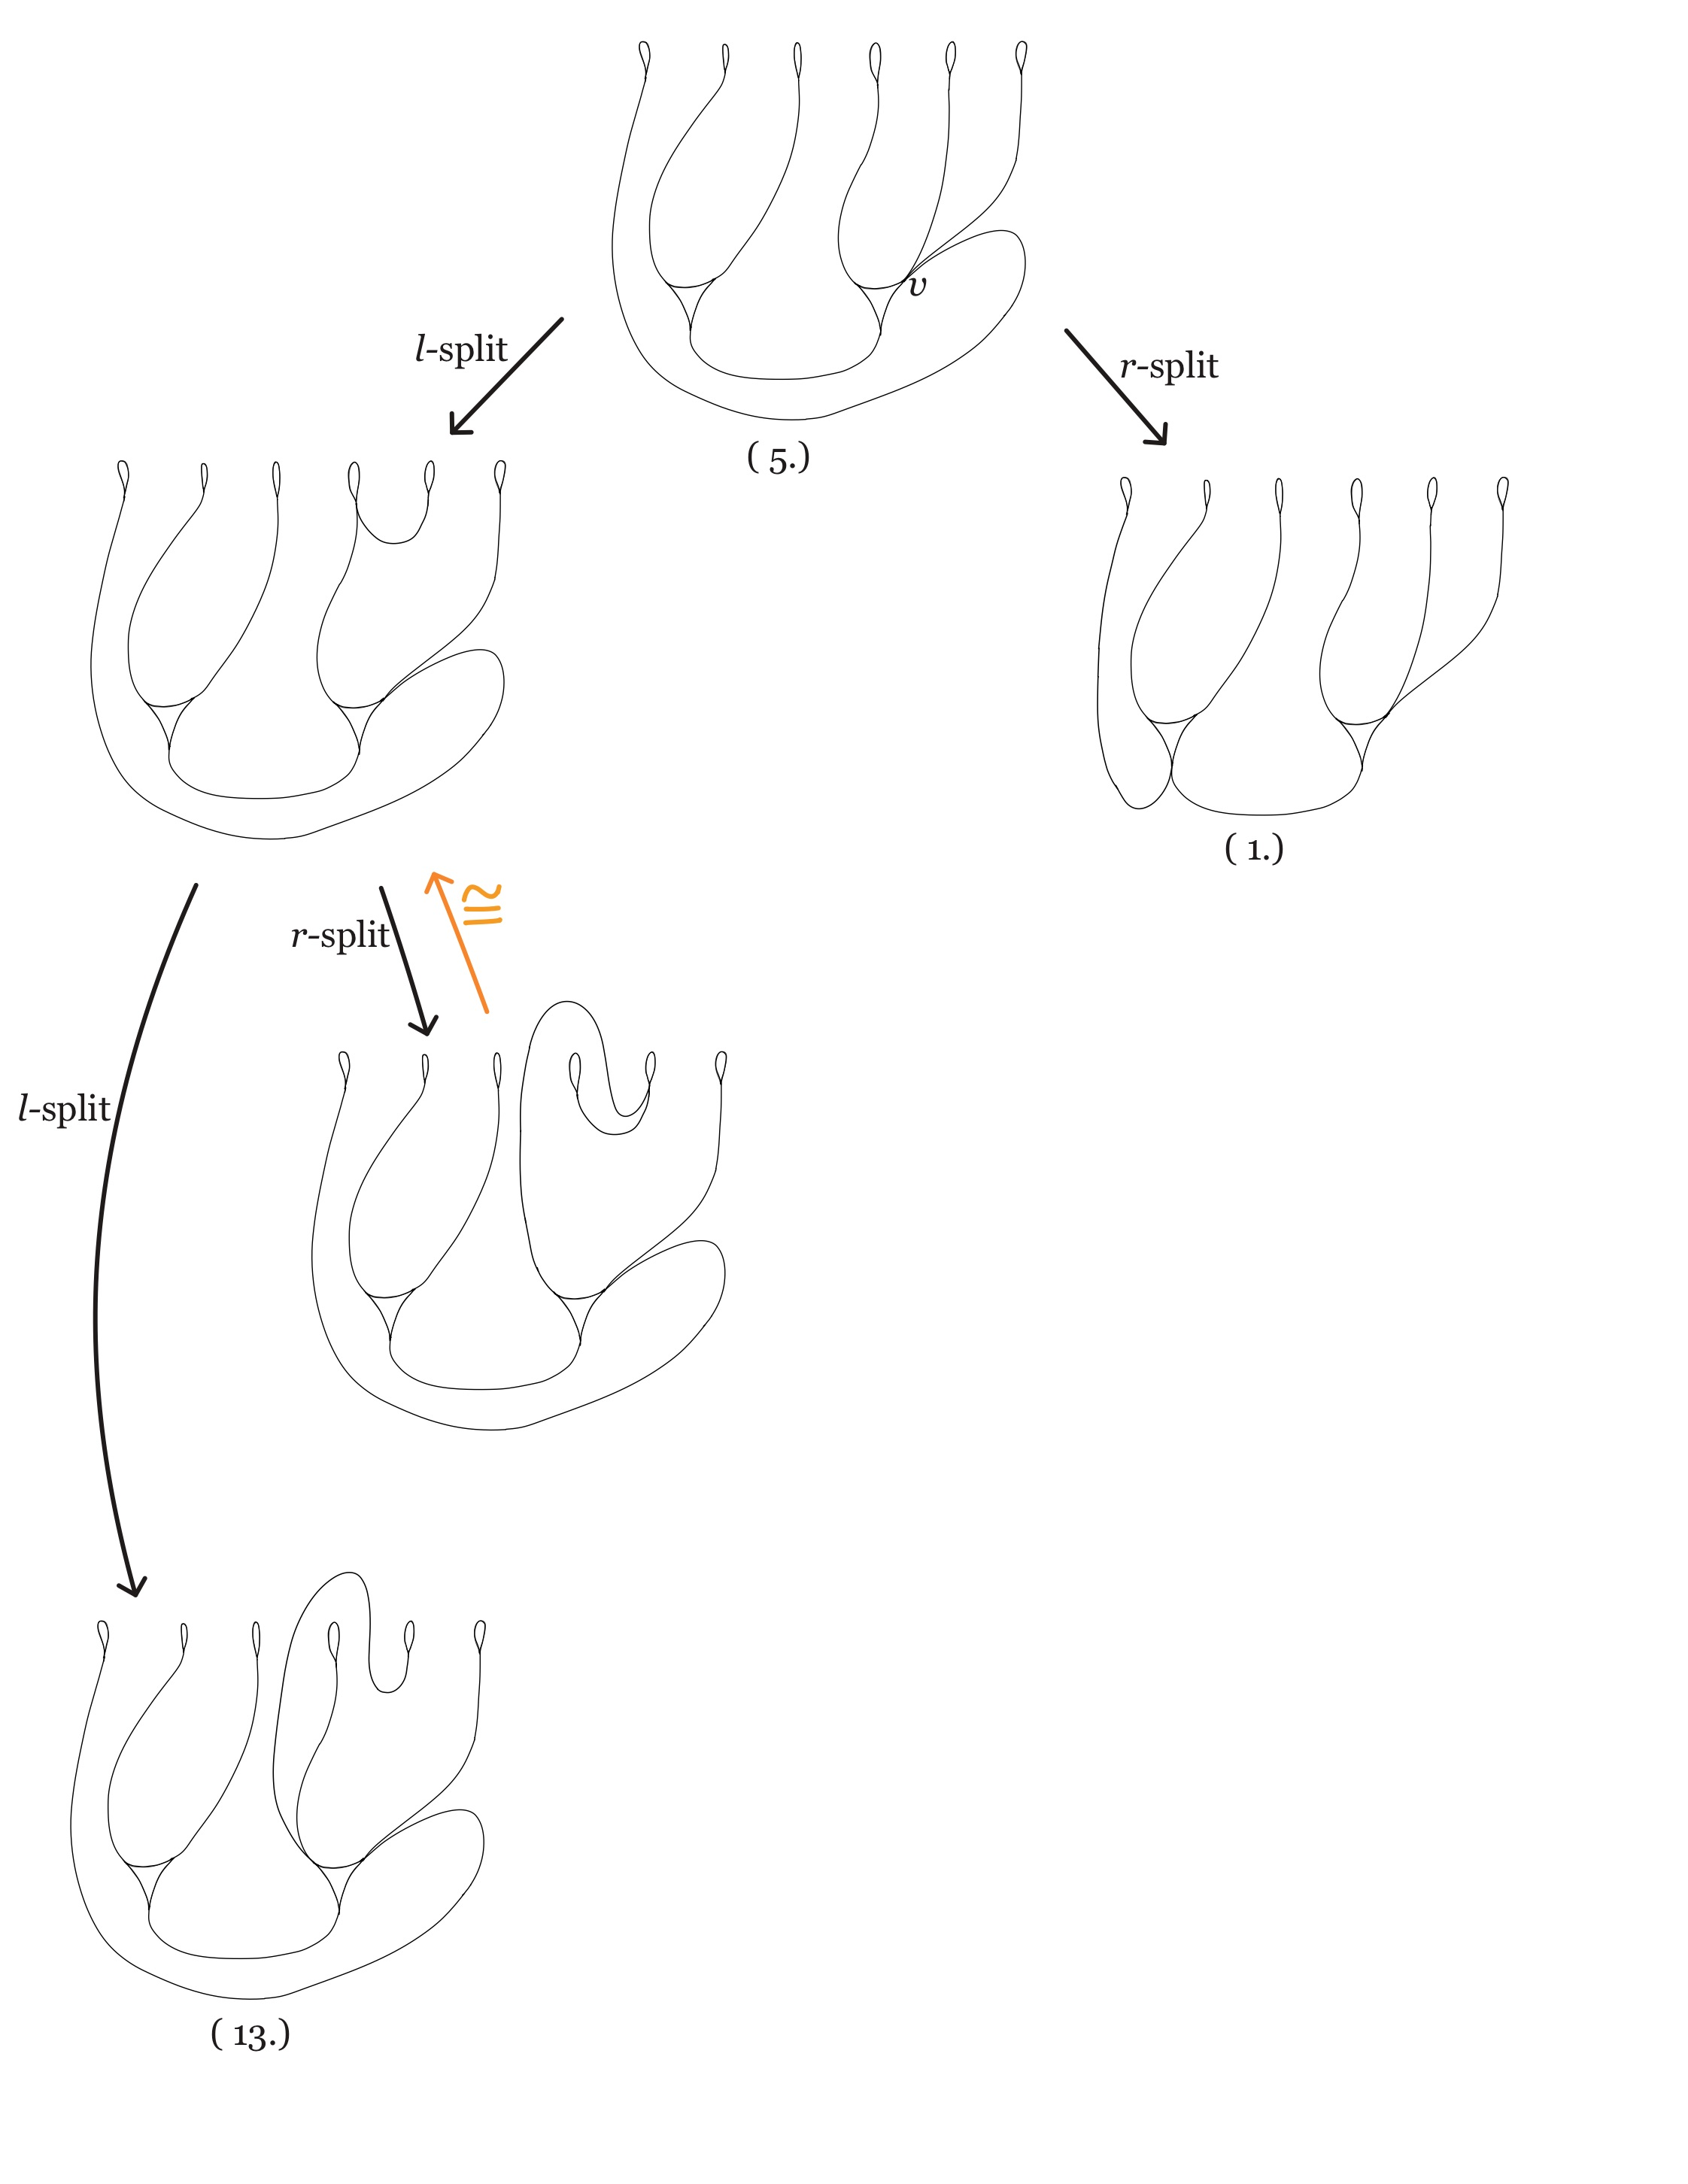
\includegraphics[width=\linewidth, height=0.45\textheight, keepaspectratio]{figures_splitting/5 Splitting.jpg}
    \caption{This splitting sequence shows train track (5.) eventually splits to the train tracks (13.) or (1.).}
    \label{fig:7_splitting}
\end{figure*}

\begin{figure*}[p] % [p] forces this to be on its own page, which is often necessary for large figures
    \centering
    % Restrict height to 45% of the text block per image, maintaining aspect ratio
    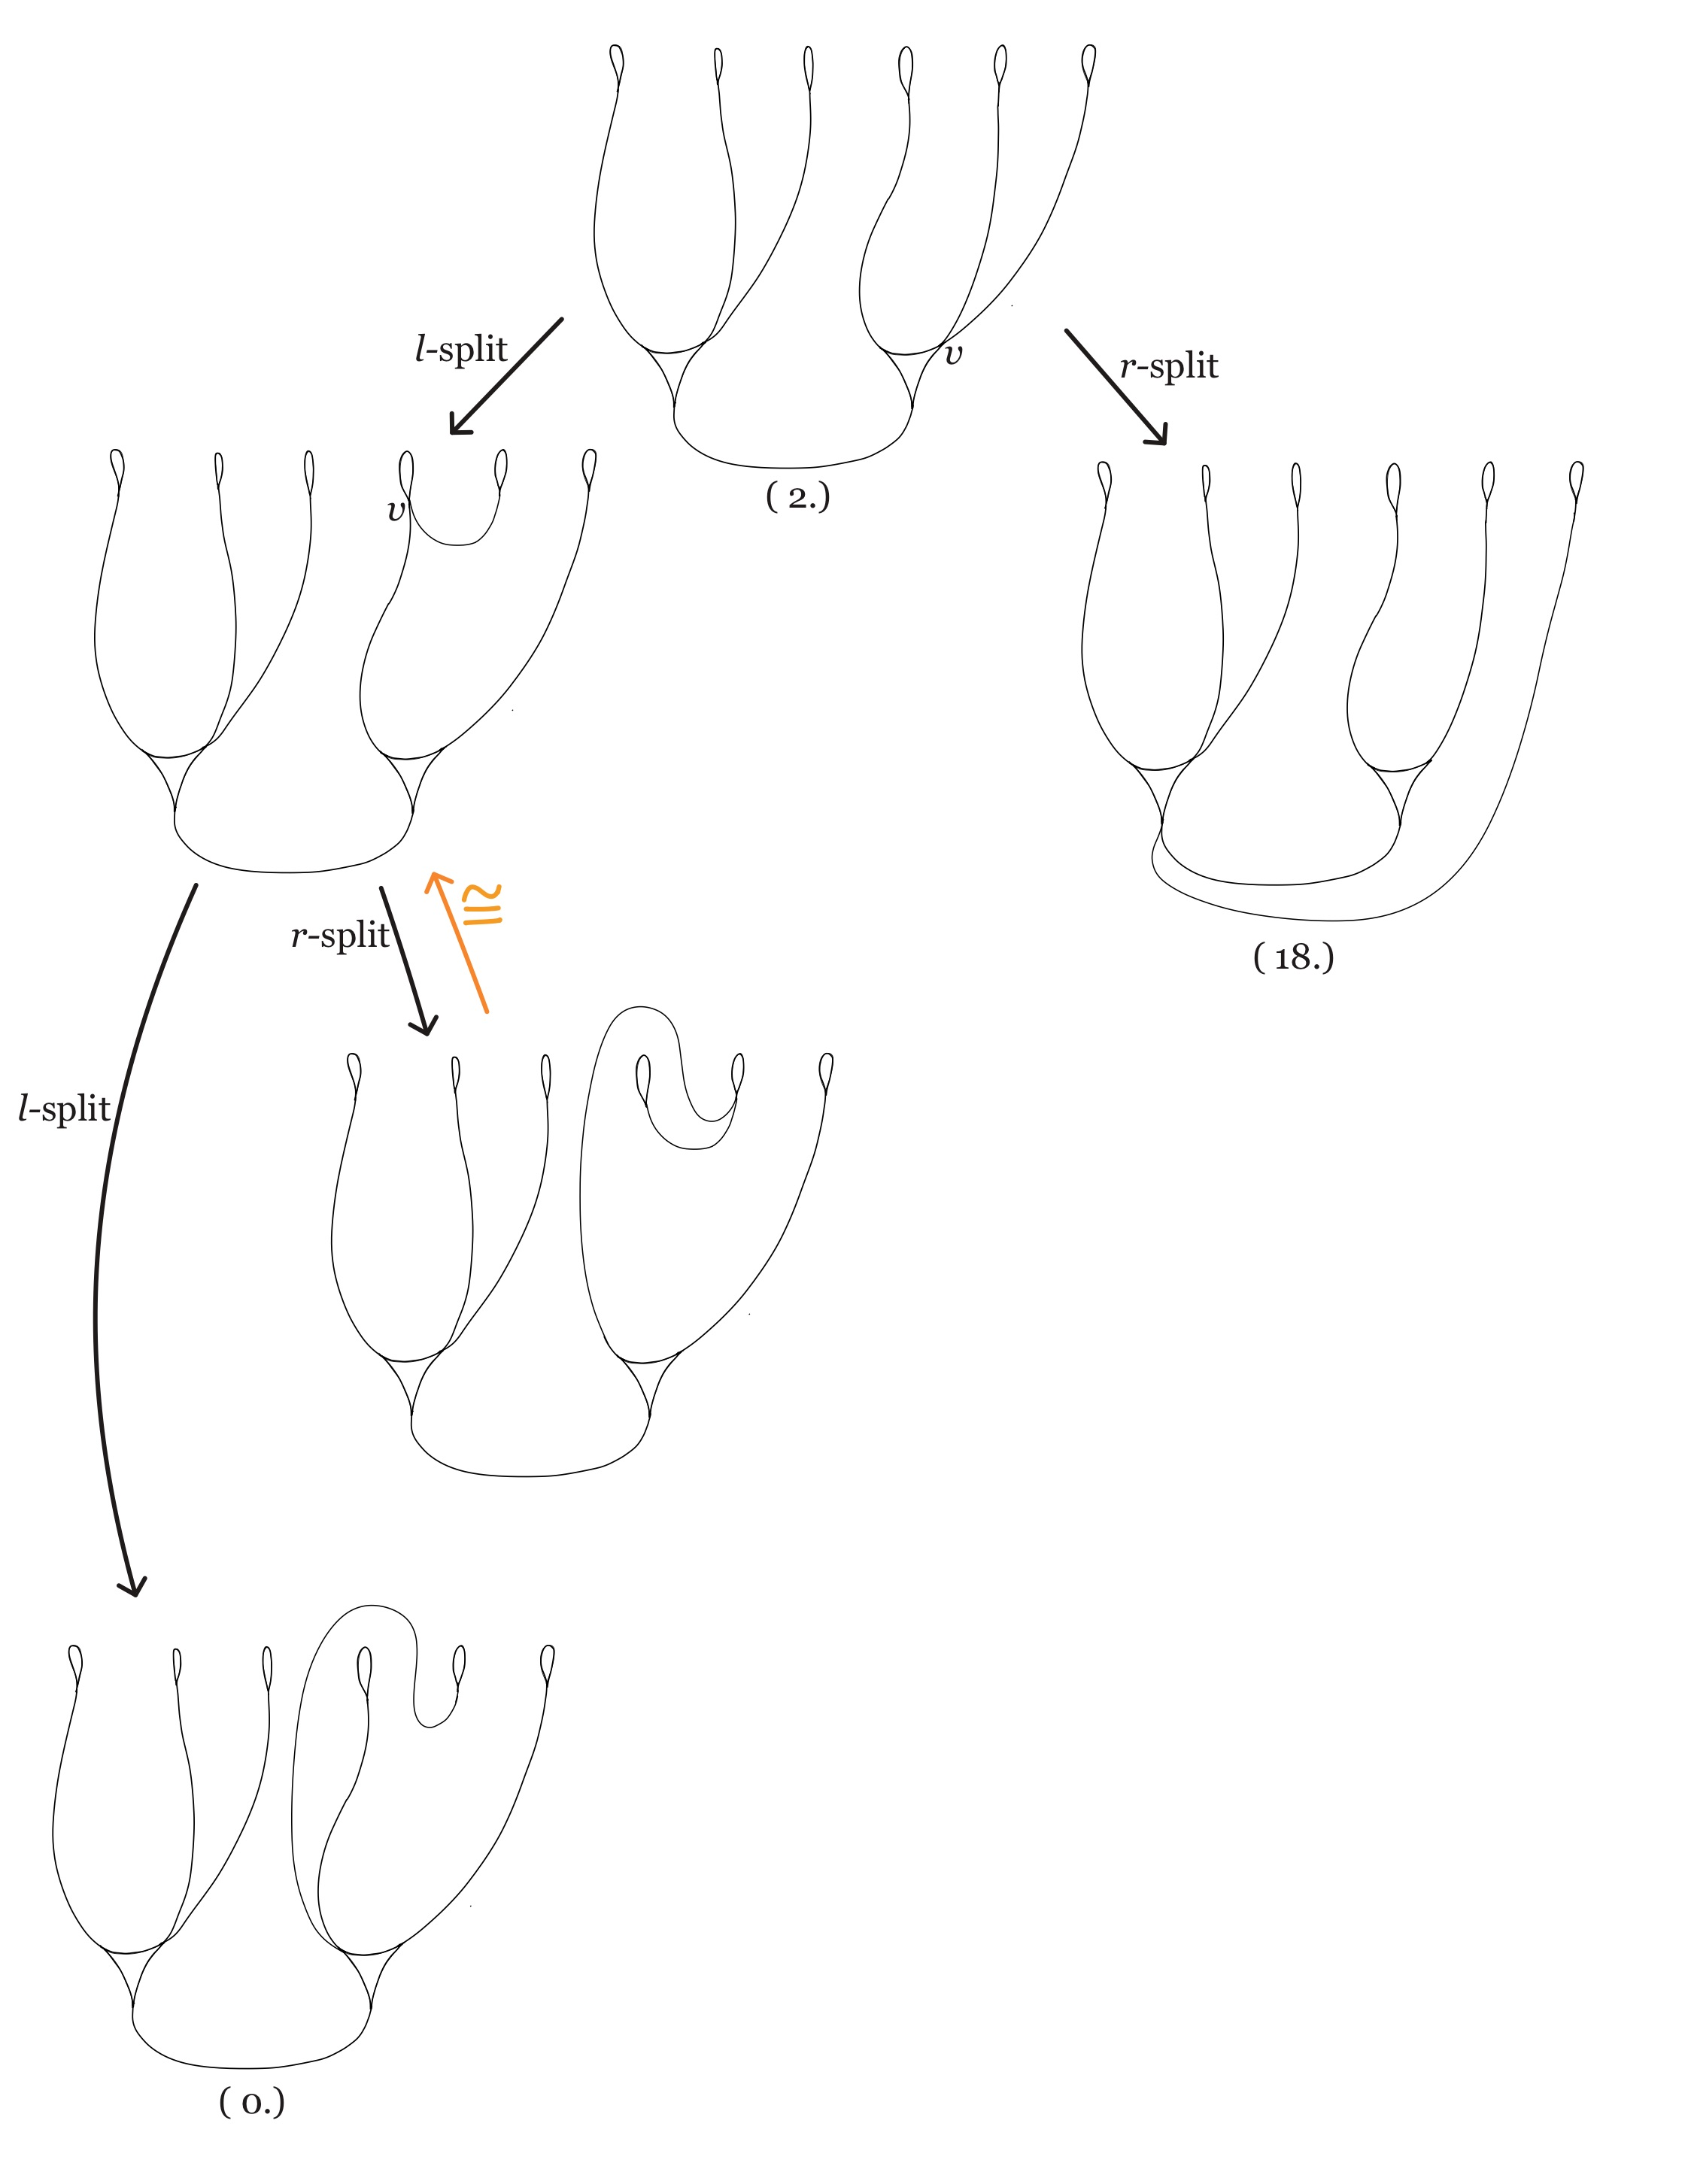
\includegraphics[width=\linewidth, height=0.45\textheight, keepaspectratio]{figures_splitting/2 Splitting-1.jpg}\\[0pt]
    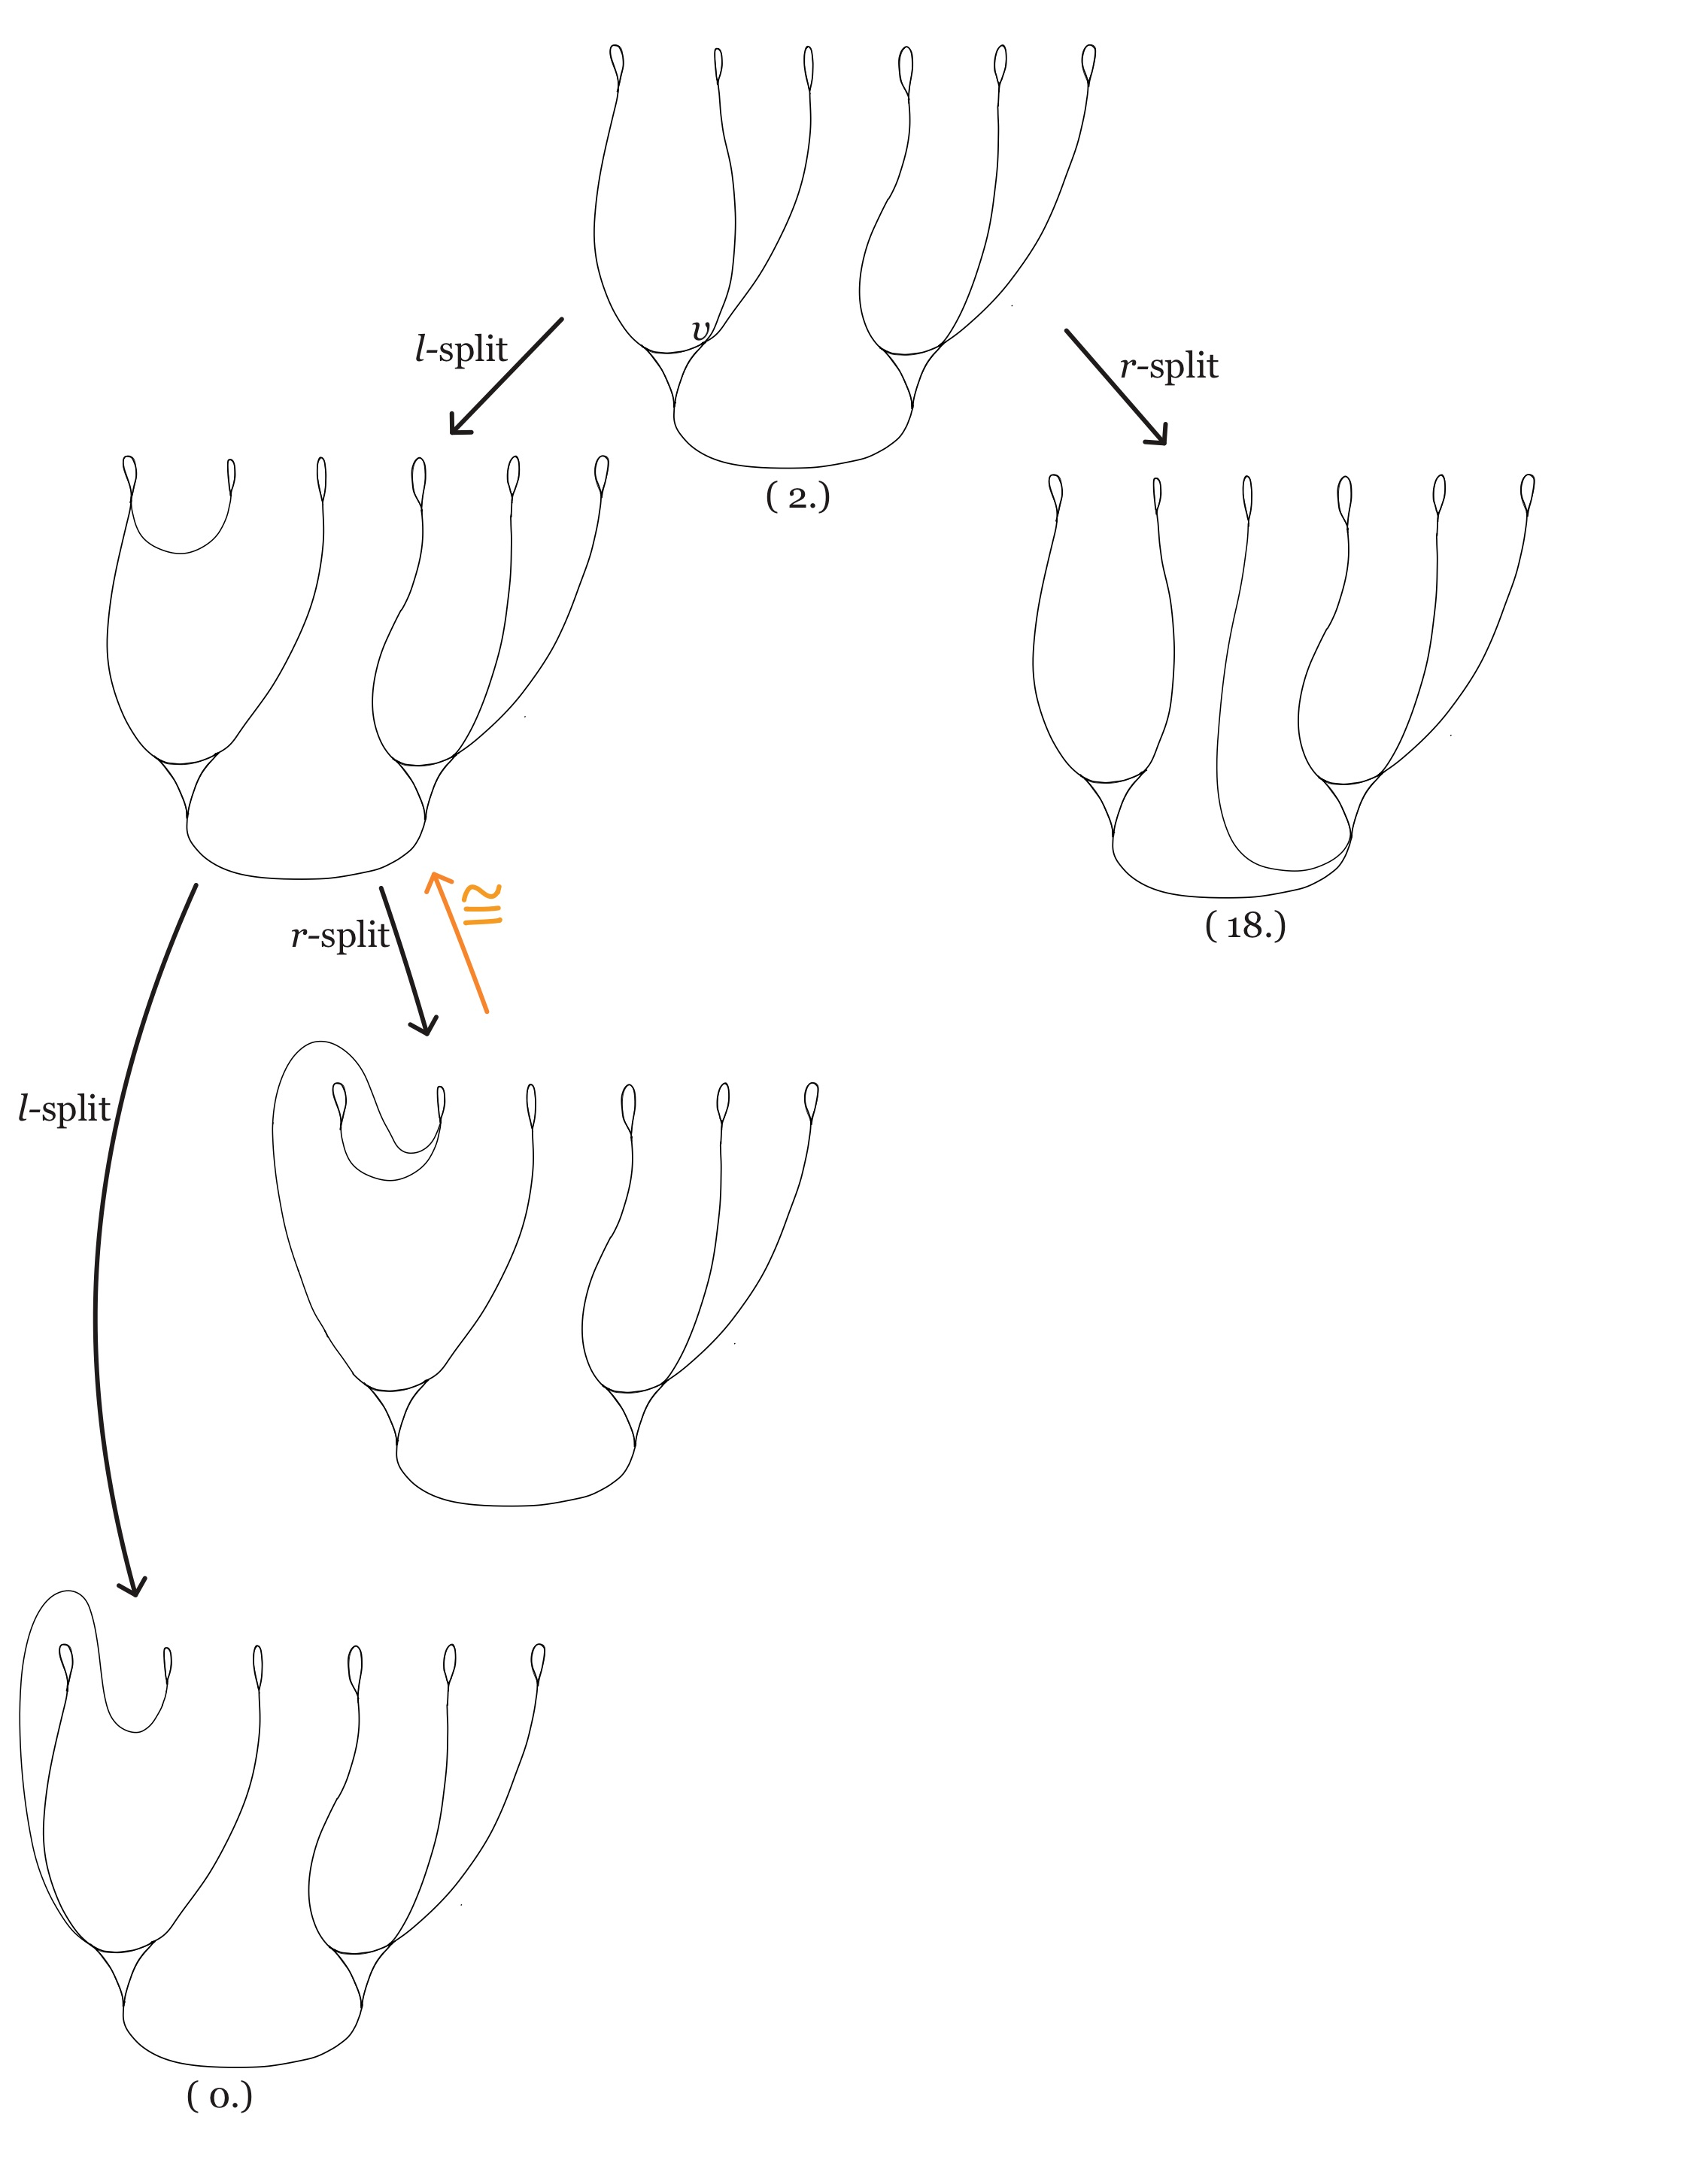
\includegraphics[width=\linewidth, height=0.45\textheight, keepaspectratio]{figures_splitting/2 Splitting-2.jpg}
    \caption{This splitting sequence shows train track (2.) eventually splits to the train tracks (18.) or (0.).}
    \label{fig:8_splitting}
\end{figure*}

\begin{figure*}[p] % [p] forces this to be on its own page, which is often necessary for large figures
    \centering
    % Restrict height to 45% of the text block per image, maintaining aspect ratio
    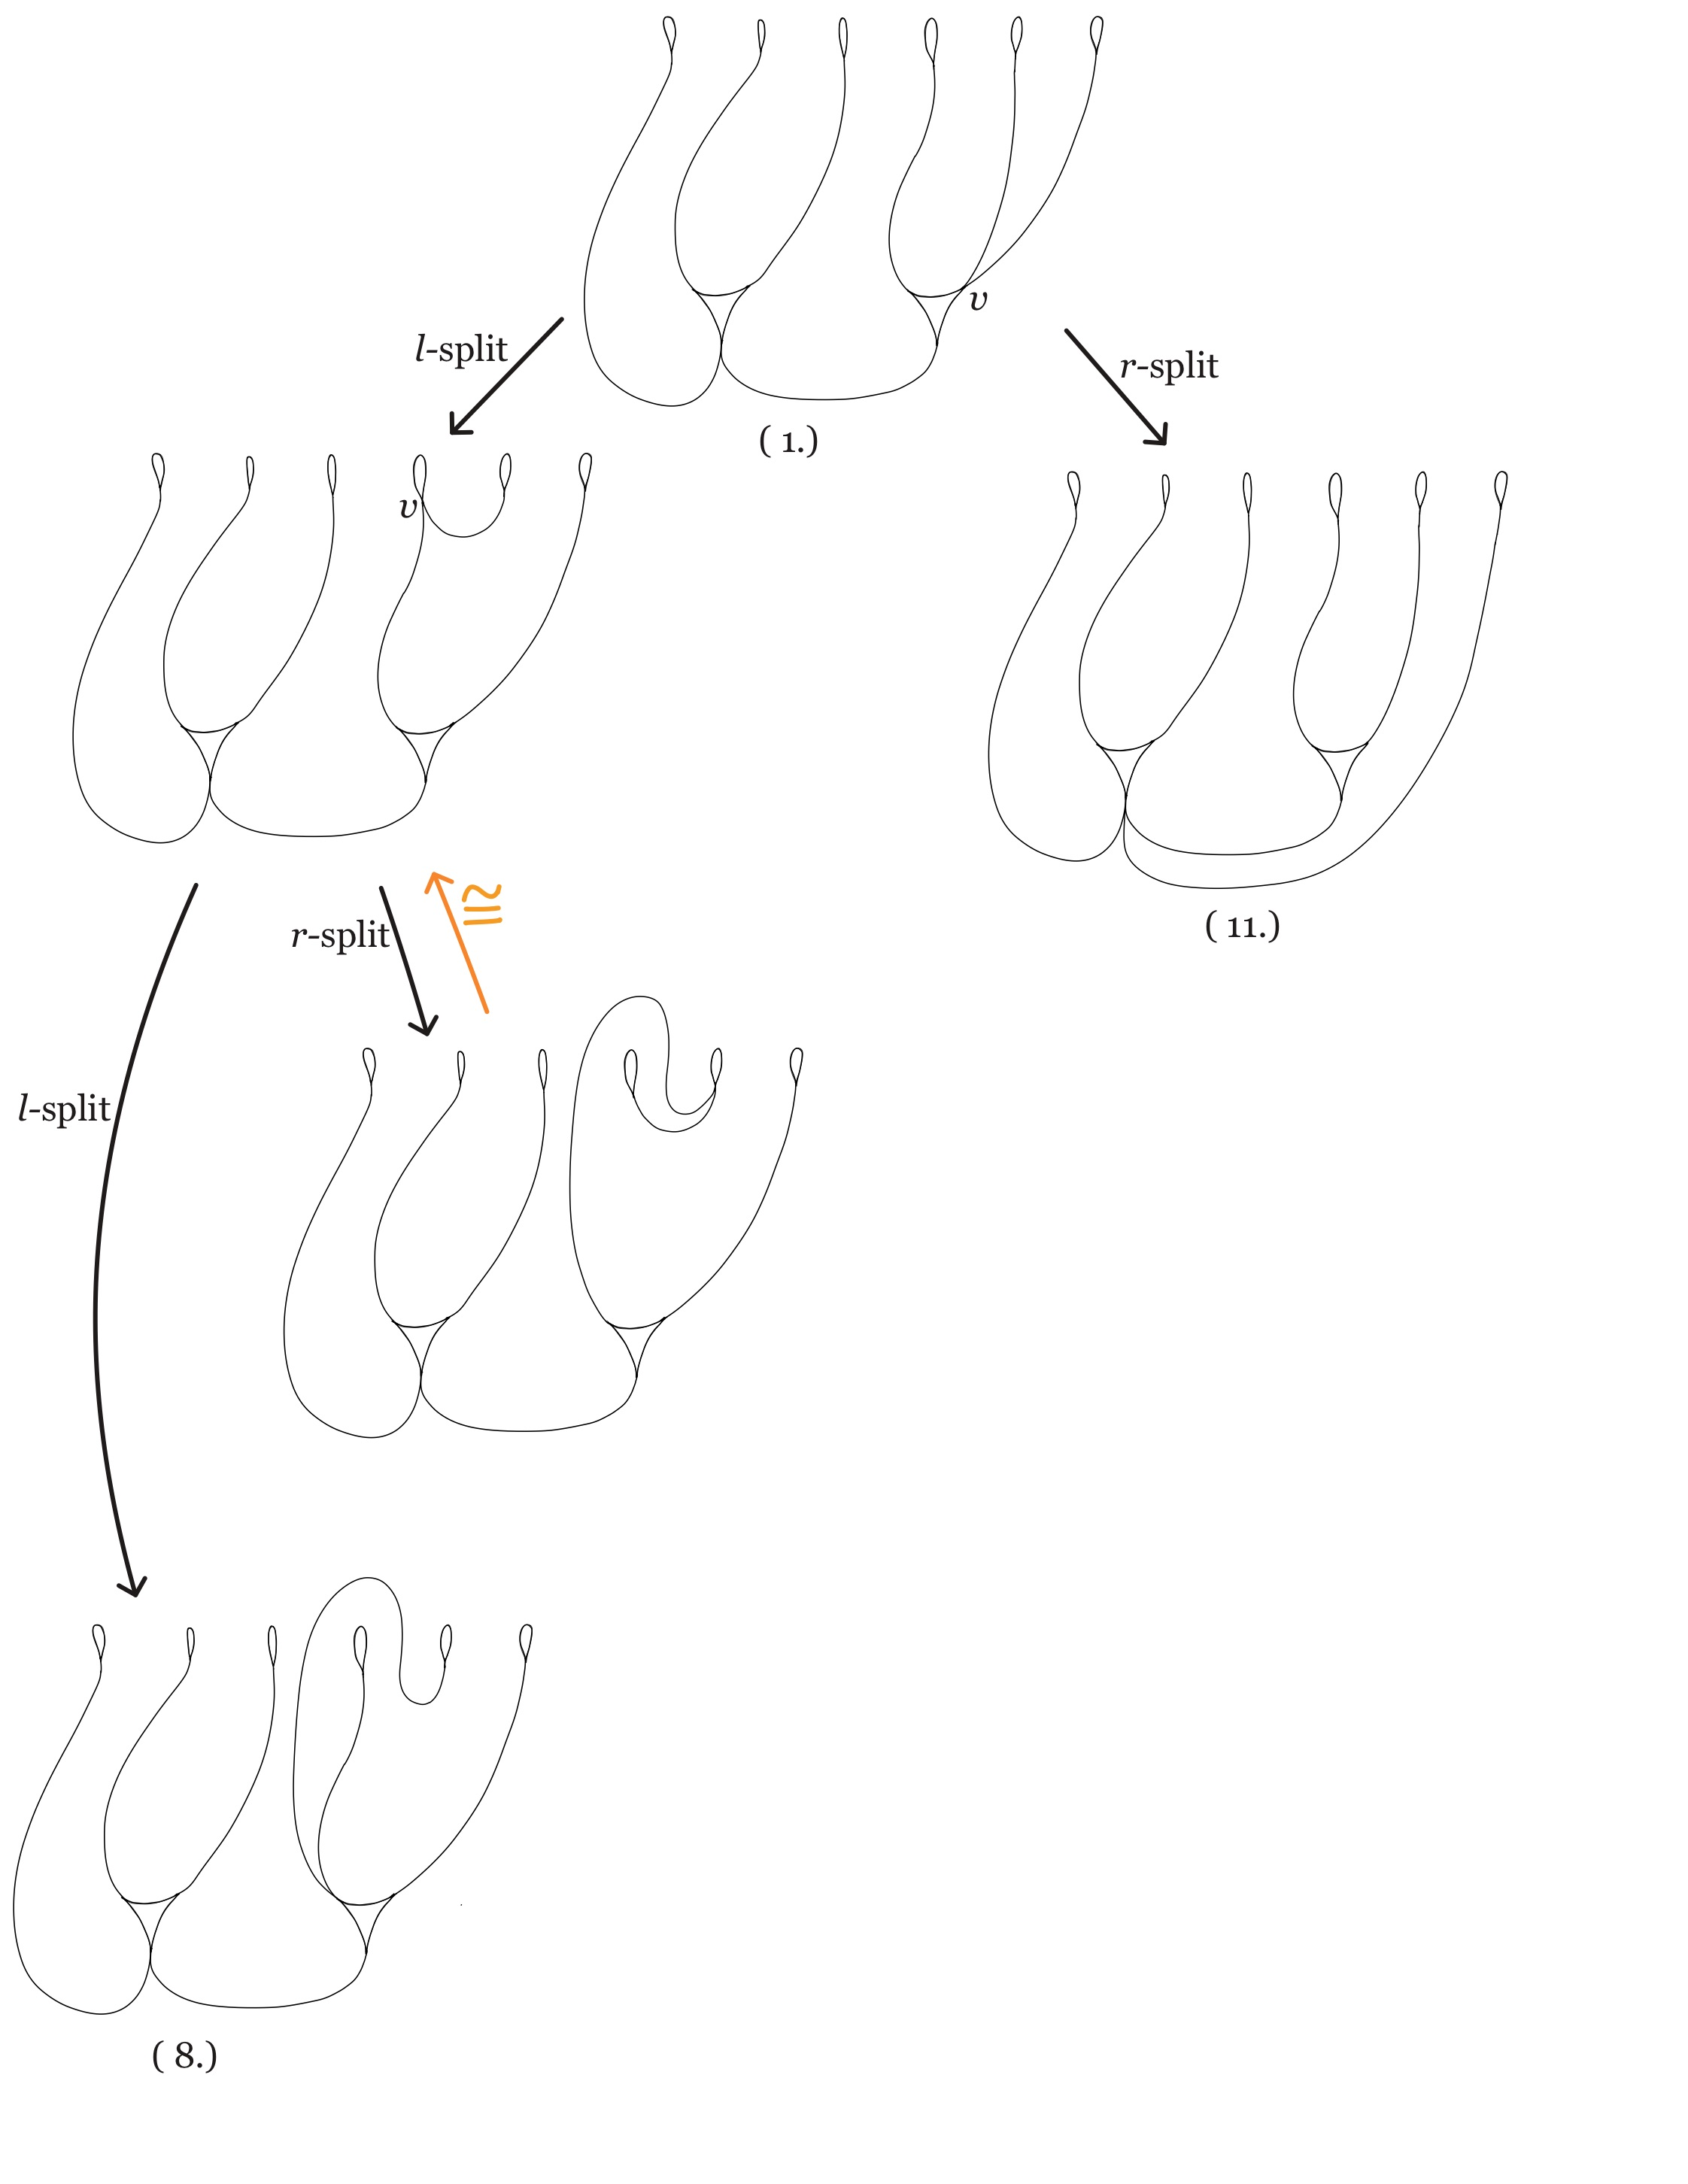
\includegraphics[width=\linewidth, height=0.45\textheight, keepaspectratio]{figures_splitting/1 Splitting-1.jpg}\\[0pt]
    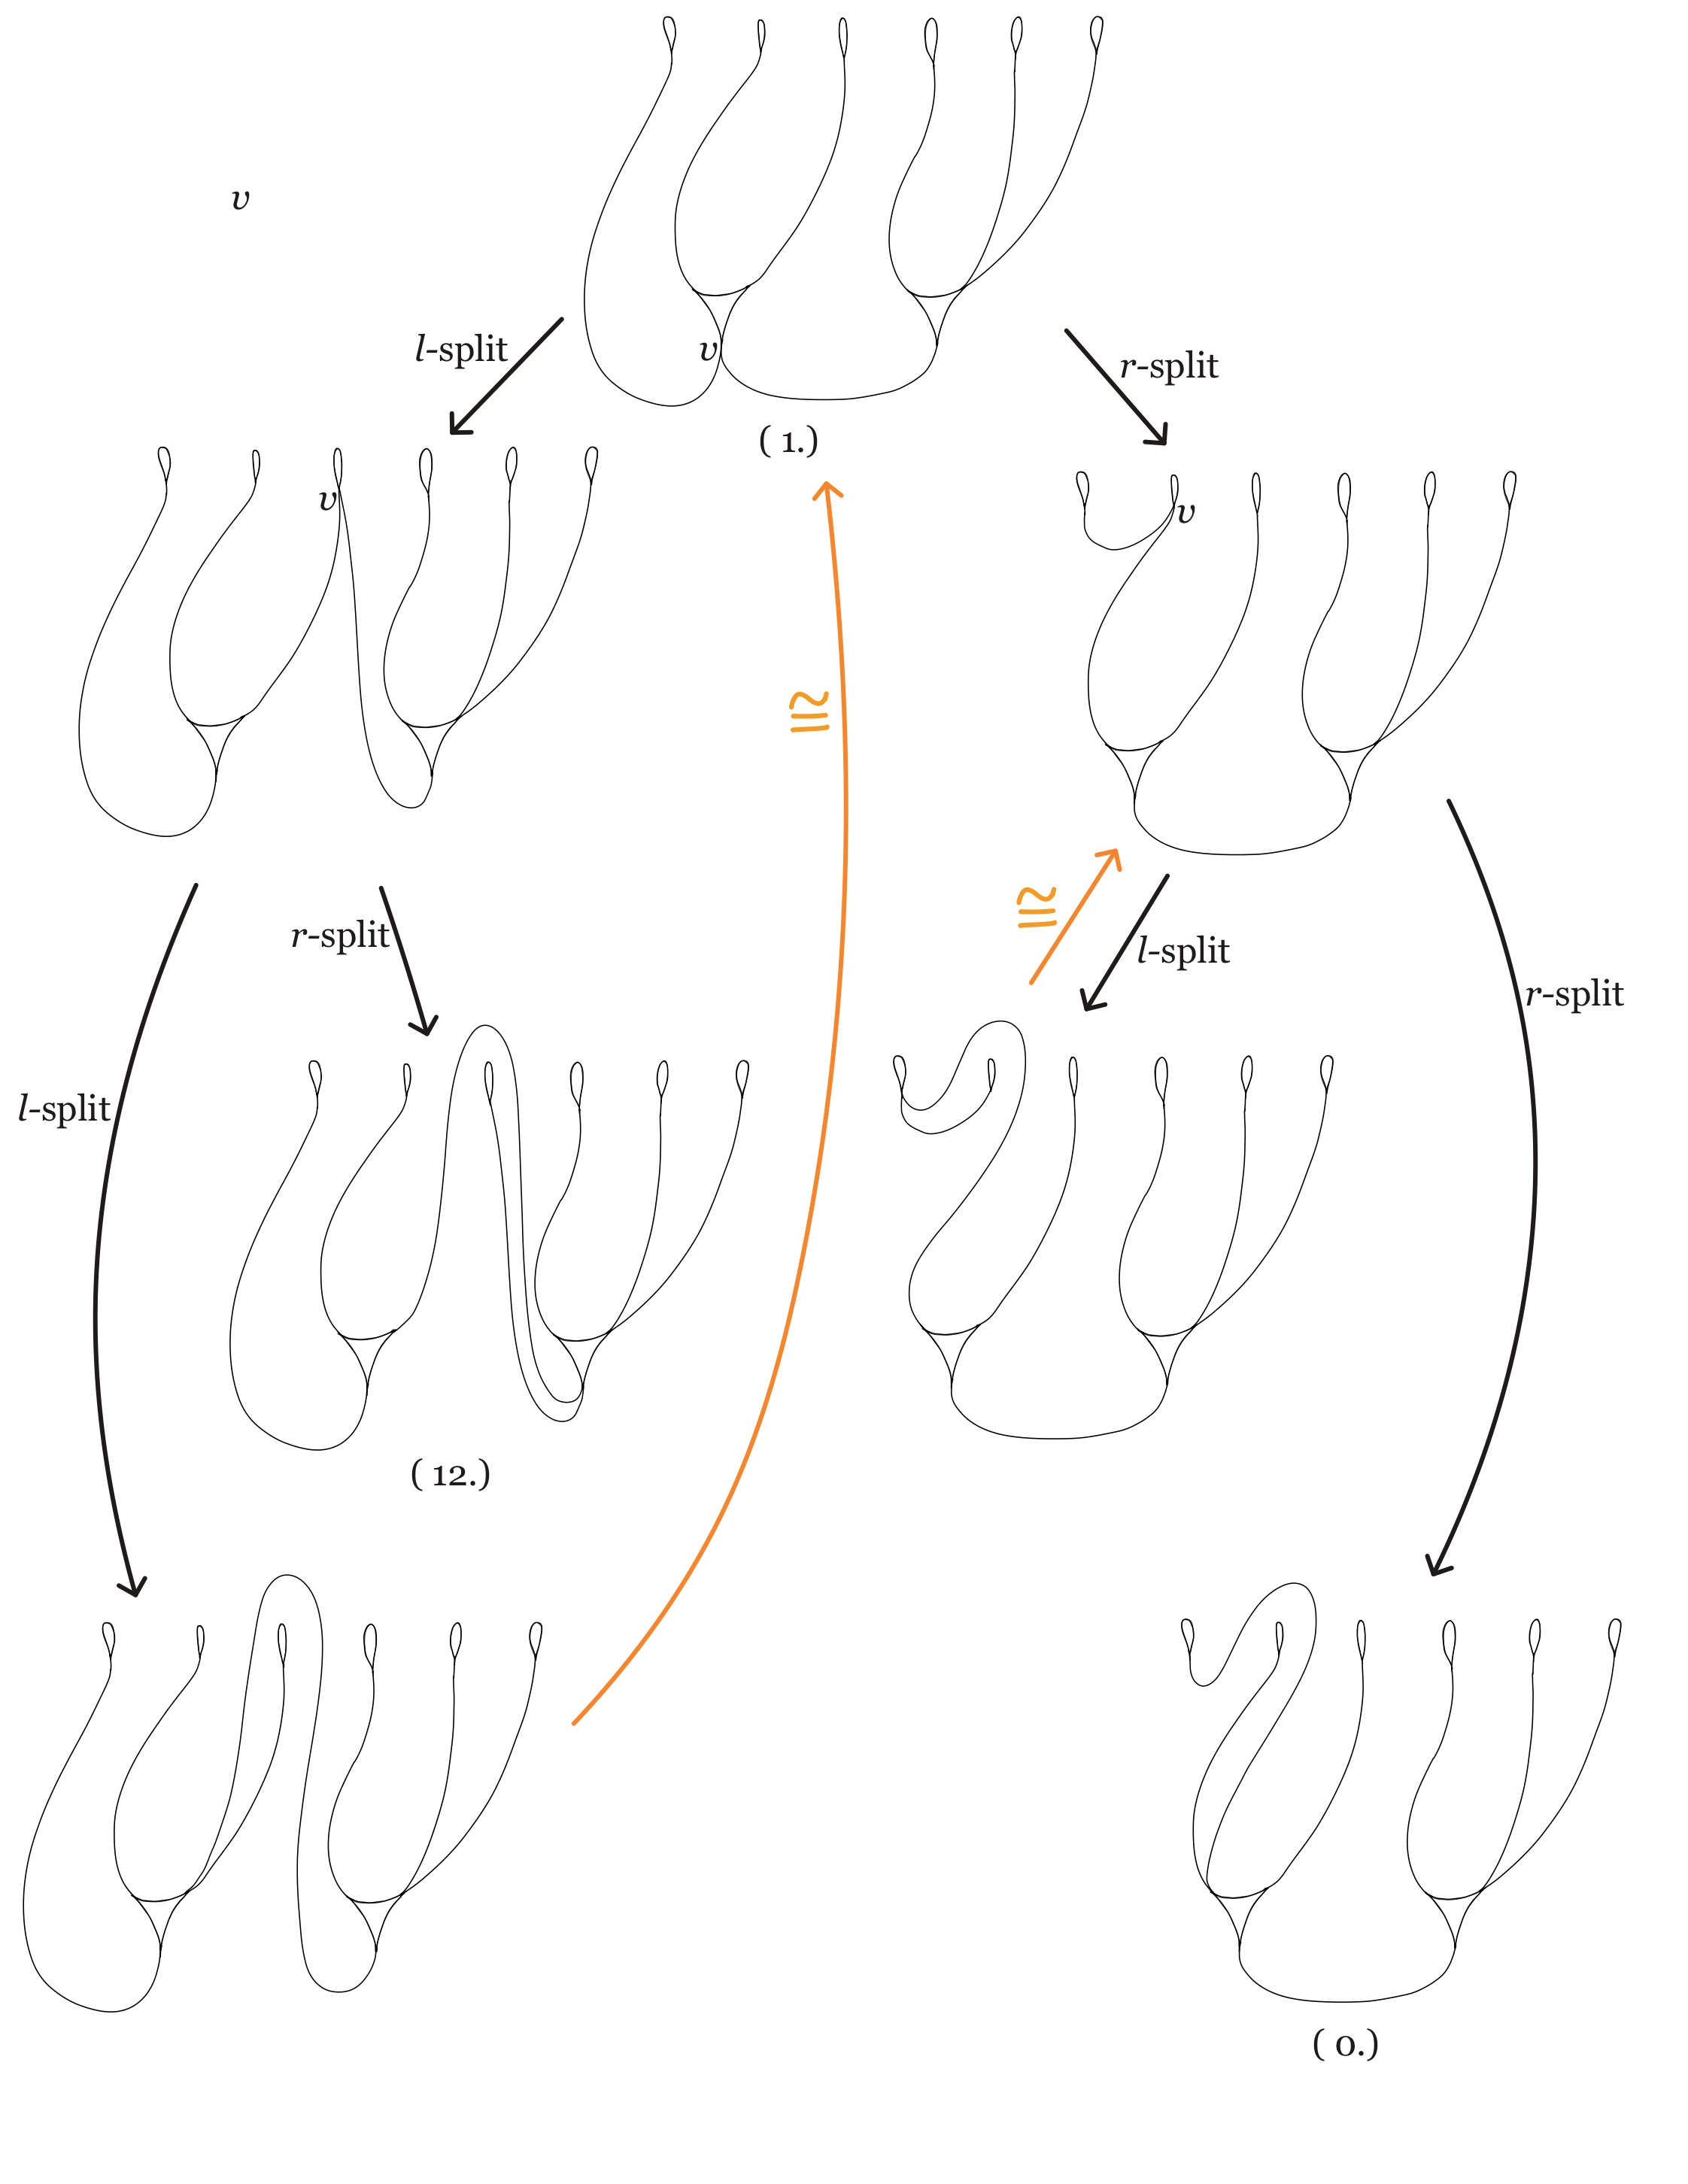
\includegraphics[width=\linewidth, height=0.45\textheight, keepaspectratio]{figures_splitting/1 Splitting-2.jpg}
    \caption{This splitting sequence shows train track (1.) eventually splits to the train tracks (11.), (8.), (12.), or (0.).}
    \label{fig:8_splitting}
\end{figure*}